% Options for packages loaded elsewhere
\PassOptionsToPackage{unicode}{hyperref}
\PassOptionsToPackage{hyphens}{url}
%
\documentclass[
]{article}
\usepackage{lmodern}
\usepackage{amsmath}
\usepackage{ifxetex,ifluatex}
\ifnum 0\ifxetex 1\fi\ifluatex 1\fi=0 % if pdftex
  \usepackage[T1]{fontenc}
  \usepackage[utf8]{inputenc}
  \usepackage{textcomp} % provide euro and other symbols
  \usepackage{amssymb}
\else % if luatex or xetex
  \usepackage{unicode-math}
  \defaultfontfeatures{Scale=MatchLowercase}
  \defaultfontfeatures[\rmfamily]{Ligatures=TeX,Scale=1}
\fi
% Use upquote if available, for straight quotes in verbatim environments
\IfFileExists{upquote.sty}{\usepackage{upquote}}{}
\IfFileExists{microtype.sty}{% use microtype if available
  \usepackage[]{microtype}
  \UseMicrotypeSet[protrusion]{basicmath} % disable protrusion for tt fonts
}{}
\makeatletter
\@ifundefined{KOMAClassName}{% if non-KOMA class
  \IfFileExists{parskip.sty}{%
    \usepackage{parskip}
  }{% else
    \setlength{\parindent}{0pt}
    \setlength{\parskip}{6pt plus 2pt minus 1pt}}
}{% if KOMA class
  \KOMAoptions{parskip=half}}
\makeatother
\usepackage{xcolor}
\IfFileExists{xurl.sty}{\usepackage{xurl}}{} % add URL line breaks if available
\IfFileExists{bookmark.sty}{\usepackage{bookmark}}{\usepackage{hyperref}}
\hypersetup{
  pdftitle={UP 494 Final Project- An Introductory Data Inventory for Unionville's Assets and Challenges},
  pdfauthor={Will Finkelstein, MUP1.},
  hidelinks,
  pdfcreator={LaTeX via pandoc}}
\urlstyle{same} % disable monospaced font for URLs
\usepackage[margin=1in]{geometry}
\usepackage{color}
\usepackage{fancyvrb}
\newcommand{\VerbBar}{|}
\newcommand{\VERB}{\Verb[commandchars=\\\{\}]}
\DefineVerbatimEnvironment{Highlighting}{Verbatim}{commandchars=\\\{\}}
% Add ',fontsize=\small' for more characters per line
\usepackage{framed}
\definecolor{shadecolor}{RGB}{248,248,248}
\newenvironment{Shaded}{\begin{snugshade}}{\end{snugshade}}
\newcommand{\AlertTok}[1]{\textcolor[rgb]{0.94,0.16,0.16}{#1}}
\newcommand{\AnnotationTok}[1]{\textcolor[rgb]{0.56,0.35,0.01}{\textbf{\textit{#1}}}}
\newcommand{\AttributeTok}[1]{\textcolor[rgb]{0.77,0.63,0.00}{#1}}
\newcommand{\BaseNTok}[1]{\textcolor[rgb]{0.00,0.00,0.81}{#1}}
\newcommand{\BuiltInTok}[1]{#1}
\newcommand{\CharTok}[1]{\textcolor[rgb]{0.31,0.60,0.02}{#1}}
\newcommand{\CommentTok}[1]{\textcolor[rgb]{0.56,0.35,0.01}{\textit{#1}}}
\newcommand{\CommentVarTok}[1]{\textcolor[rgb]{0.56,0.35,0.01}{\textbf{\textit{#1}}}}
\newcommand{\ConstantTok}[1]{\textcolor[rgb]{0.00,0.00,0.00}{#1}}
\newcommand{\ControlFlowTok}[1]{\textcolor[rgb]{0.13,0.29,0.53}{\textbf{#1}}}
\newcommand{\DataTypeTok}[1]{\textcolor[rgb]{0.13,0.29,0.53}{#1}}
\newcommand{\DecValTok}[1]{\textcolor[rgb]{0.00,0.00,0.81}{#1}}
\newcommand{\DocumentationTok}[1]{\textcolor[rgb]{0.56,0.35,0.01}{\textbf{\textit{#1}}}}
\newcommand{\ErrorTok}[1]{\textcolor[rgb]{0.64,0.00,0.00}{\textbf{#1}}}
\newcommand{\ExtensionTok}[1]{#1}
\newcommand{\FloatTok}[1]{\textcolor[rgb]{0.00,0.00,0.81}{#1}}
\newcommand{\FunctionTok}[1]{\textcolor[rgb]{0.00,0.00,0.00}{#1}}
\newcommand{\ImportTok}[1]{#1}
\newcommand{\InformationTok}[1]{\textcolor[rgb]{0.56,0.35,0.01}{\textbf{\textit{#1}}}}
\newcommand{\KeywordTok}[1]{\textcolor[rgb]{0.13,0.29,0.53}{\textbf{#1}}}
\newcommand{\NormalTok}[1]{#1}
\newcommand{\OperatorTok}[1]{\textcolor[rgb]{0.81,0.36,0.00}{\textbf{#1}}}
\newcommand{\OtherTok}[1]{\textcolor[rgb]{0.56,0.35,0.01}{#1}}
\newcommand{\PreprocessorTok}[1]{\textcolor[rgb]{0.56,0.35,0.01}{\textit{#1}}}
\newcommand{\RegionMarkerTok}[1]{#1}
\newcommand{\SpecialCharTok}[1]{\textcolor[rgb]{0.00,0.00,0.00}{#1}}
\newcommand{\SpecialStringTok}[1]{\textcolor[rgb]{0.31,0.60,0.02}{#1}}
\newcommand{\StringTok}[1]{\textcolor[rgb]{0.31,0.60,0.02}{#1}}
\newcommand{\VariableTok}[1]{\textcolor[rgb]{0.00,0.00,0.00}{#1}}
\newcommand{\VerbatimStringTok}[1]{\textcolor[rgb]{0.31,0.60,0.02}{#1}}
\newcommand{\WarningTok}[1]{\textcolor[rgb]{0.56,0.35,0.01}{\textbf{\textit{#1}}}}
\usepackage{graphicx}
\makeatletter
\def\maxwidth{\ifdim\Gin@nat@width>\linewidth\linewidth\else\Gin@nat@width\fi}
\def\maxheight{\ifdim\Gin@nat@height>\textheight\textheight\else\Gin@nat@height\fi}
\makeatother
% Scale images if necessary, so that they will not overflow the page
% margins by default, and it is still possible to overwrite the defaults
% using explicit options in \includegraphics[width, height, ...]{}
\setkeys{Gin}{width=\maxwidth,height=\maxheight,keepaspectratio}
% Set default figure placement to htbp
\makeatletter
\def\fps@figure{htbp}
\makeatother
\setlength{\emergencystretch}{3em} % prevent overfull lines
\providecommand{\tightlist}{%
  \setlength{\itemsep}{0pt}\setlength{\parskip}{0pt}}
\setcounter{secnumdepth}{-\maxdimen} % remove section numbering
\ifluatex
  \usepackage{selnolig}  % disable illegal ligatures
\fi

\title{UP 494 Final Project- An Introductory Data Inventory for
Unionville's Assets and Challenges}
\author{Will Finkelstein, MUP1.}
\date{5/10/2021}

\begin{document}
\maketitle

{
\setcounter{tocdepth}{2}
\tableofcontents
}
For my Neighborhood Analysis course this semester, I wanted to develop a
data engagement framework for addressing the perennial disconnect
between data sets and accessible application. While this still defines
the longterm approach, the steps in this first analysis are to introduce
the stories and resilience of Macon's Unionville Neighborhood, while
doing some basic analyses to determine potential relationships between
two major geographic data sets. The data pertain to 2020 crime
statistics and the quantity and response times related to resident-filed
maintenance requests, filed using the SeeClickFix application. These two
sets, given at the county commission District 5 level (not the original
plan, but see limitations for more!), have data pertaining to Unionville
at the street level and contain information pertaining to the two major,
consistently highlighted resident worries. Typical to underrepresented,
majority-black neigbhorhoods, blight, dumping, and other issues of
community neglect are also a major concern in Unionville. Many crime
headlines, a major reputation for gang activity, and a city-county-wide
police shortage also highlight the public safety fears that many
residents continue to face. These analyses aim to determine if the
existing data show a relationship between crime and see-click-fix
requests, while also inferring what might be missing from discussions of
community health. Afterwards, a brief plan for engagement and othr next
stps is shared.

\#Context and Background

Unionville is a historically black, traditionally working class
neighborhood in the ``near west side'' of Macon. It is located just
across I-75 from Mercer University. Mercer has funded a lot of real
estate and foundational grant programs that spill into a few
``higher-need'' neighborhoods proximate to downtown, partially to permit
its continued development agenda. As Unionville is just outside of that
extended ``downtown'' area, the neighborhood is unable to access these.

Unionville has continued to transition from being a majority-homeowner
community to having a declining older homeowner, mostly renter
population. Children, having left long ago and having little interest in
holding onto their aging parents' homes, would sell these to any
interested buyer. This trend throughout the community has enabled
slumlords. Blight, illegal dumping, and high renter turnover have been
constant norms. Additionally, Unionville has had a reputation for gang
activity and violent crime since my early childhood. Without going too
deep into specific incidents, a significant number of last year's
shootings occurred close to hear. A number of neighborhood commercial
buildings have murals paying homage to community pillars who were
victims of gun violence. And the Bentley \& Sons Funeral Home, easily
its most renowned neighborhood institution, provides free services for
the families of victims as a social impact program. Yet, there are
stories of unity outside of struggle also. Former Mayor C. Jack Ellis,
Macon's first and only black mayor, began his civic career as a
community organizer in Unionville. The Frank Johnson Community Center,
operated by Parks \& Recreation, recently received around \$1 million
worth of renovations from SPLOST (Special Purpose Local Option Sales
Tax) revenues (Dunlap, 2017). The Macon-Bibb County Government's new
Public Works and Neighborhood Cleanup Collaborations consider Unionville
a major priority (Macon-Bibb County, 2021). And the neighborhood's
small, but strong business community takes a serious interest in seeing
the change happen.

The remainder of this final will introduce the questions of analysis,
the spatial areas of analysis (tracts and streets), the data sources in
use, clear limitations, and the next steps for a final product. While
the initial plan was to conduct further analysis on qualitative
perspectives from long-term residents and neighborhood leaders, some
communication challenges with organizers and other time constraints make
that unfeasible at present. The expectations for how to better engage
the community will be in the form of an extension, briefly described at
the end.

First, we will get our R console ready:

\begin{Shaded}
\begin{Highlighting}[]
 \FunctionTok{library}\NormalTok{(tidyverse)}
\end{Highlighting}
\end{Shaded}

\begin{verbatim}
## -- Attaching packages --------------------------------------- tidyverse 1.3.0 --
\end{verbatim}

\begin{verbatim}
## v ggplot2 3.3.3     v purrr   0.3.4
## v tibble  3.0.5     v dplyr   1.0.3
## v tidyr   1.1.2     v stringr 1.4.0
## v readr   1.4.0     v forcats 0.5.1
\end{verbatim}

\begin{verbatim}
## -- Conflicts ------------------------------------------ tidyverse_conflicts() --
## x dplyr::filter() masks stats::filter()
## x dplyr::lag()    masks stats::lag()
\end{verbatim}

\begin{Shaded}
\begin{Highlighting}[]
\FunctionTok{library}\NormalTok{(tidycensus)}
\FunctionTok{library}\NormalTok{(tidyr)}
\FunctionTok{library}\NormalTok{(qdapRegex)}
\end{Highlighting}
\end{Shaded}

\begin{verbatim}
## Warning: package 'qdapRegex' was built under R version 4.0.5
\end{verbatim}

\begin{verbatim}
## 
## Attaching package: 'qdapRegex'
\end{verbatim}

\begin{verbatim}
## The following object is masked from 'package:dplyr':
## 
##     explain
\end{verbatim}

\begin{verbatim}
## The following object is masked from 'package:ggplot2':
## 
##     %+%
\end{verbatim}

\begin{Shaded}
\begin{Highlighting}[]
\FunctionTok{census\_api\_key}\NormalTok{(}\StringTok{"f6d3f308f00a0ffda3aa19e86807e0ea5960d86e"}\NormalTok{, }\AttributeTok{install =} \ConstantTok{TRUE}\NormalTok{, }\AttributeTok{overwrite=}\ConstantTok{TRUE}\NormalTok{) }
\end{Highlighting}
\end{Shaded}

\begin{verbatim}
## Your original .Renviron will be backed up and stored in your R HOME directory if needed.
\end{verbatim}

\begin{verbatim}
## Your API key has been stored in your .Renviron and can be accessed by Sys.getenv("CENSUS_API_KEY"). 
## To use now, restart R or run `readRenviron("~/.Renviron")`
\end{verbatim}

\begin{verbatim}
## [1] "f6d3f308f00a0ffda3aa19e86807e0ea5960d86e"
\end{verbatim}

\#Questions Guiding Investigation The two major questions that this
analysis seeks to answer are as follows:

\begin{enumerate}
\def\labelenumi{\arabic{enumi}.}
\tightlist
\item
  Do quantity and response time to user submitted government service
  requests made with SeeClickFix have any relation to crime rate?
\item
  What do these variables tell us about neighborhood health?
\end{enumerate}

\hypertarget{methods-and-approach}{%
\section{Methods and Approach}\label{methods-and-approach}}

For this ongoing project, I am conducting analyses that occur at three
spatial scales. One analysis occurs countywide, which evaluates the
relationship between ``Median Household Income'' and ``Proportion of
Population that is Black/African American'' in every census tract in
Bibb County, Georgia. This is at a single point in time, but draws the
picture of whether current sociodemographic data reflect trends
consistent with other places.A table and dot map will be included, with
each entry corresponding to a Census Tract. This is Macon-Bibb County's
location compared to the rest of Georgia, with interstates and larger
cities also highlighted:

There is some confusion about the light intensity, but Macon-Bibb has
been considered the fourth largest community in Georgia since its 2014
consolidation. Compared to other notable major cities, Macon-Bibb is
located about 80 miles southeast of Atlanta, 100 miles east of Columbus,
120 miles southwest of Augusta, 170 miles northwest of Savannah, and 90
miles southwest of Athens.

Next, Census Tract 104, which contains almost all of Unionville and a
couple of blocks of Napier Heights neighborhood, will be compared to two
other Census Tracts in the same county commission district. These are
Census Tract 101, which contains all of Macon's Pleasant Hill
neighborhood located between downtown and the near-west side, and Census
Tract 102, which represents the Historic Vineville Neighborhood and is
located just west of Pleasant Hill and a mile north of Unionville. Prior
to the construction of Interstate 75 and neighborhood physical split in
the mid-20th century, Pleasant Hill was Macon's most well-to-do black
neighborhood. This neighborhood is a bit more diverse, but majority
white (65\%) Both of these border Macon's central business district.
Occupancy rates and median household incomes are evaluated over a five
year period (2015-19) for these three tracts, to hopefully determine if
connection to downtown investment opportunities has begun to cause a
revitalization. Tracts 101, 102, and 104 are shown below, as are the
boundaries of District 5. There is a star marking my childhood home:

\begin{Shaded}
\begin{Highlighting}[]
\NormalTok{ knitr}\SpecialCharTok{::}\FunctionTok{include\_graphics}\NormalTok{(}\StringTok{"Tract Comparison.png"}\NormalTok{)}
\end{Highlighting}
\end{Shaded}

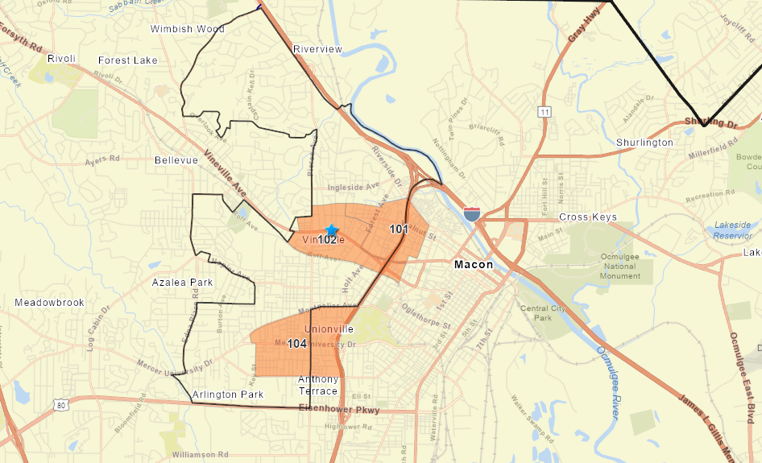
\includegraphics{Tract Comparison.png}

\begin{Shaded}
\begin{Highlighting}[]
\CommentTok{\#Map Made with ARCGIS Online}
\CommentTok{\#Source: (ESRI, 2021; Atlanta Regional Commission, 2020; Nabhan, 2018)}
\end{Highlighting}
\end{Shaded}

You might notice that the tracts and district boundaries are not
contiguous. This mismatch, contributing to two inconsistent levels of
analysis, involves being given a different data set than originall
requested. This will be discussed further in the limitations section
below.

The final level of analysis occurs entirely in Census Tract 104. The
plan is to evaluate a potential relationship by road between Public
Works Department response times to reported property neglect and the
number of crimes to occur in 2020 on each road. The strongest precedent
to the work is consistent reporting that a clear majority of
Macon-Bibb's record breaking 51 homicides occurred in Unionville (Hicks,
2020). The following map visualizes Census Tract 104 close up, also
indicating built barriers (interstate, university) that separate this
from the larger area considered downtown:

\begin{Shaded}
\begin{Highlighting}[]
\NormalTok{knitr}\SpecialCharTok{::}\FunctionTok{include\_graphics}\NormalTok{(}\StringTok{"unionvillemap.png"}\NormalTok{)}
\end{Highlighting}
\end{Shaded}

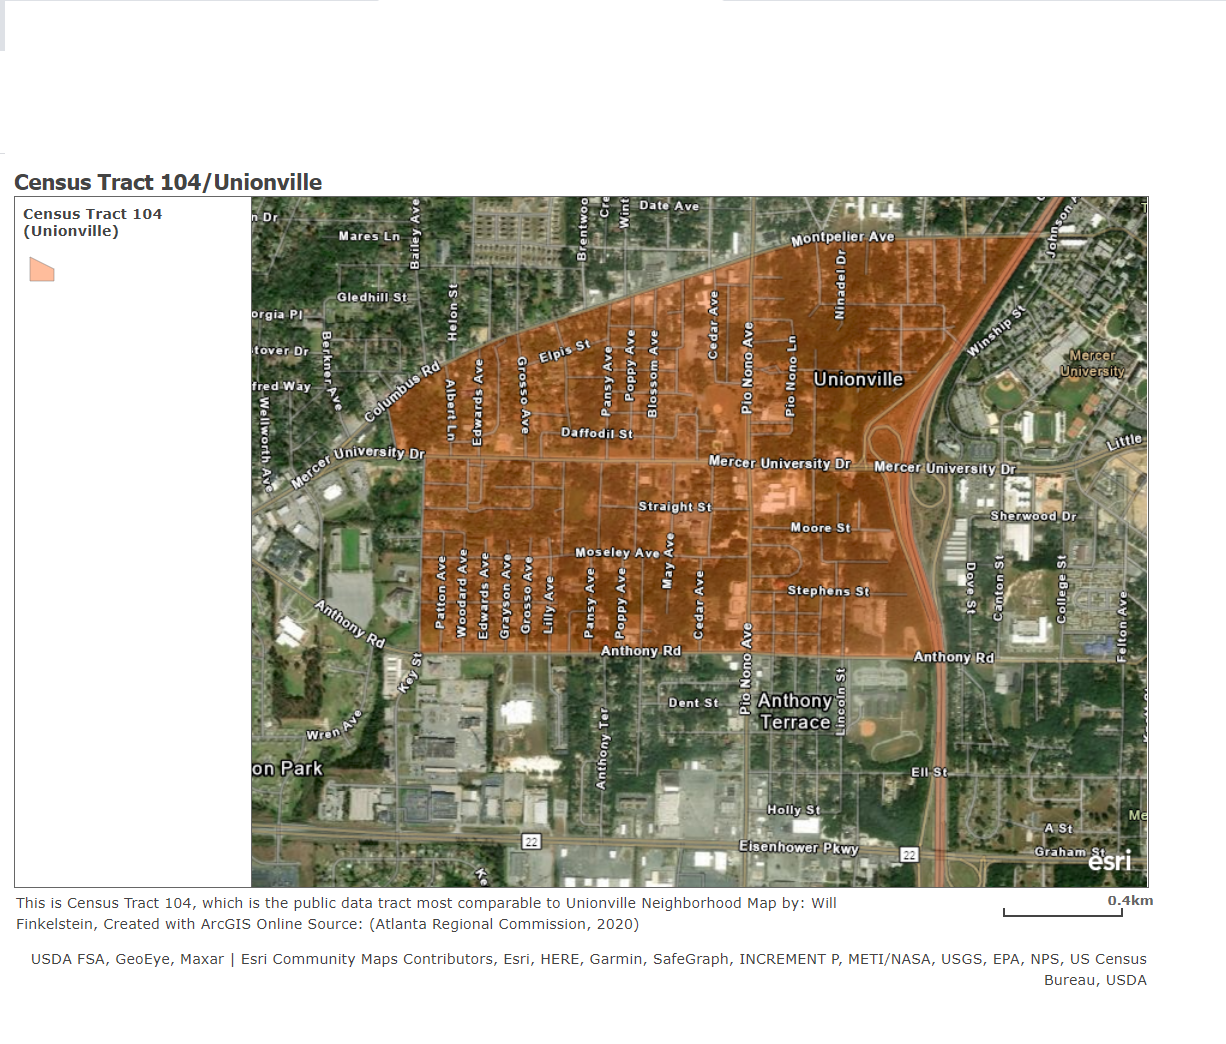
\includegraphics{unionvillemap.png} The data is still in process for
this. But after evaluating these at the street level, tract-wide
response times to crime rates may be compared with Tracts 101 and 138 as
well.

\hypertarget{data-sources}{%
\section{Data Sources}\label{data-sources}}

The county wide and three tract comparative analyses rely on ACS 5 year
data from the US census Bureau. These include Table B19013 (Median
Household Income), Table B02001 (Race), and Table DP04 (Housing
Characteristics) for years 2015, 2016, 2017, 2018, 2019. After importing
selected variables, values are added using mutate for certain variables
such as year and percentage black.

Data for the final street by street analysis in Unionville utilized sets
imported from agencies within the consolidated Macon-Bibb County
government. Crime data for 2020 came from the ``highly understaffed''
Bibb County Sheriff's office and data for SeeClickFix requests and
response times came from the county's Office of Communications.
``SeeClickFix'' allows residents to report instances of property
neglect, lack of code enforcement, illegal dumping, and various other
situations of public neglect. Complaints go into the potential scopes of
eight government departments. These are Solid Waste and its privatized
partner for residential trash disposal (ADS), Traffic, Recreation,
Public Works, Facilities Management, Code Enforcement, Animal Services,
Beautification (MaconBibb.us, 2021).

\#Limitations The following three situations represented significant
limitations to the original analysis vision. These all pose important
implications for future work in this context and others.

1.Data quality- It took over a month from the request date to receive
the SeeClickFix and crime data and the geographic data was highly
inconsistent. While the original plan had been to receive data at the
tract level for Census Tracts 101, 104, and 138 (in East Macon, often
considered part of the downtown core), the data I received pertained to
the Macon-Bibb county commission district 5. While most of Pleasant Hill
and Unionville are located in this area, parts are left out so the
comparative scale is inconsistent. I am not entirely sure if this was on
me for not clarifying what I needed, but it requires levels of analysis
to be at different scales. In analyses where the data are strictly tract
level (first part, from the Census), geographic inputs are Census Tracts
101, 102, and 104. But for the crime and SeeClickFix service requests,
the data pertain to neighborhoods listed as Pleasant Hill (PH),
Vineville (V), and Unionville (U). They largely cover the same areas,
but the transition is imperfect.

\begin{enumerate}
\def\labelenumi{\arabic{enumi}.}
\setcounter{enumi}{1}
\item
  Engagement Inability- While the initial undertaking was supposed to be
  first stage ``asset-challenge inventory'', my inability to reach the
  couple of related organizers that I knew or ability to meet others who
  lived here limited this. The approach I chose instead was to look at
  indicators that are discussed as pressing publicly, do some analyses,
  and proceed to take this to the community before discussing a clear
  course of action.
\item
  Imperfect variable substitution- Using response times to services
  requests and vacancy rates to predict the presence of blight in a
  neighborhood are an imperfect, and largely incomplete, approach. Yet,
  the lack of clear data to show the interplay between housing
  indicators and human impacts prevent us from having something cleaner.
  Like the geographic scale inconsistencies, it is worth mentioning that
  these have wholes but can hopefully point to similar situations that
  blight poses.
\end{enumerate}

\#Analyses

While waiting for local data, I went ahead and utilized Census data to
connect county-wide and three tract comparisons.

After running code and plotting the relationship between ``Median
Household Income'' and ``Proportion of Population that is Black/African
American'' in every census tract in Bibb County, Georgia, I got the
following table:

\begin{Shaded}
\begin{Highlighting}[]
\NormalTok{maconbibbmhi\_2019 }\OtherTok{\textless{}{-}} \FunctionTok{get\_acs}\NormalTok{(}\AttributeTok{geography =} \StringTok{"tract"}\NormalTok{, }\AttributeTok{state =} \StringTok{"GA"}\NormalTok{, }\AttributeTok{county =} \StringTok{"Bibb"}\NormalTok{, }\AttributeTok{table =} \StringTok{"B19013"}\NormalTok{, }\AttributeTok{year=}\DecValTok{2019}\NormalTok{, }\AttributeTok{survey=}\StringTok{"acs5"}\NormalTok{, }\AttributeTok{output=}\StringTok{"wide"}\NormalTok{) }\SpecialCharTok{\%\textgreater{}\%}
\FunctionTok{select}\NormalTok{(NAME, B19013\_001E) }\SpecialCharTok{\%\textgreater{}\%}
\FunctionTok{rename}\NormalTok{(}\AttributeTok{Neighborhood =}\NormalTok{ NAME, }\AttributeTok{mhi =}\NormalTok{ B19013\_001E) }
\end{Highlighting}
\end{Shaded}

\begin{verbatim}
## Getting data from the 2015-2019 5-year ACS
\end{verbatim}

\begin{verbatim}
## Loading ACS5 variables for 2019 from table B19013. To cache this dataset for faster access to ACS tables in the future, run this function with `cache_table = TRUE`. You only need to do this once per ACS dataset.
\end{verbatim}

\begin{Shaded}
\begin{Highlighting}[]
\NormalTok{maconbibbmhi\_2019 }
\end{Highlighting}
\end{Shaded}

\begin{verbatim}
## # A tibble: 44 x 2
##    Neighborhood                                mhi
##    <chr>                                     <dbl>
##  1 Census Tract 135.04, Bibb County, Georgia 69118
##  2 Census Tract 136.03, Bibb County, Georgia 66996
##  3 Census Tract 136.04, Bibb County, Georgia 55000
##  4 Census Tract 136.05, Bibb County, Georgia 70379
##  5 Census Tract 136.06, Bibb County, Georgia 77143
##  6 Census Tract 137, Bibb County, Georgia    22439
##  7 Census Tract 138, Bibb County, Georgia    19063
##  8 Census Tract 139, Bibb County, Georgia    34261
##  9 Census Tract 135.02, Bibb County, Georgia 41523
## 10 Census Tract 123, Bibb County, Georgia    21205
## # ... with 34 more rows
\end{verbatim}

\begin{Shaded}
\begin{Highlighting}[]
\NormalTok{maconbibb\_blackpopulation\_2019 }\OtherTok{\textless{}{-}}\FunctionTok{get\_acs}\NormalTok{(}\AttributeTok{geography =} \StringTok{"tract"}\NormalTok{, }\AttributeTok{state =} \StringTok{"GA"}\NormalTok{,}\AttributeTok{county =} \StringTok{"Bibb"}\NormalTok{, }\AttributeTok{table =} \StringTok{"B02001"}\NormalTok{, }\AttributeTok{year=}\DecValTok{2019}\NormalTok{, }\AttributeTok{survey=}\StringTok{"acs5"}\NormalTok{, }\AttributeTok{output=}\StringTok{"wide"}\NormalTok{) }\SpecialCharTok{\%\textgreater{}\%} 
\FunctionTok{rename}\NormalTok{(}\AttributeTok{Neighborhood =}\NormalTok{ NAME,}
       \AttributeTok{pop\_tot=}\NormalTok{ B02001\_001E,}
       \AttributeTok{pop\_black =}\NormalTok{ B02001\_003E) }\SpecialCharTok{\%\textgreater{}\%}
 \FunctionTok{select}\NormalTok{(Neighborhood, pop\_tot, pop\_black) }\SpecialCharTok{\%\textgreater{}\%}
 \FunctionTok{mutate}\NormalTok{(}\AttributeTok{p\_black =}\NormalTok{ pop\_black}\SpecialCharTok{/}\NormalTok{pop\_tot) }\SpecialCharTok{\%\textgreater{}\%}
 \FunctionTok{select}\NormalTok{(Neighborhood, p\_black)}
\end{Highlighting}
\end{Shaded}

\begin{verbatim}
## Getting data from the 2015-2019 5-year ACS
\end{verbatim}

\begin{verbatim}
## Loading ACS5 variables for 2019 from table B02001. To cache this dataset for faster access to ACS tables in the future, run this function with `cache_table = TRUE`. You only need to do this once per ACS dataset.
\end{verbatim}

\begin{Shaded}
\begin{Highlighting}[]
\NormalTok{maconbibb\_blackpopulation\_2019}
\end{Highlighting}
\end{Shaded}

\begin{verbatim}
## # A tibble: 44 x 2
##    Neighborhood                              p_black
##    <chr>                                       <dbl>
##  1 Census Tract 135.04, Bibb County, Georgia   0.251
##  2 Census Tract 136.03, Bibb County, Georgia   0.339
##  3 Census Tract 136.04, Bibb County, Georgia   0.339
##  4 Census Tract 136.05, Bibb County, Georgia   0.555
##  5 Census Tract 136.06, Bibb County, Georgia   0.337
##  6 Census Tract 137, Bibb County, Georgia      0.585
##  7 Census Tract 138, Bibb County, Georgia      0.946
##  8 Census Tract 139, Bibb County, Georgia      0.464
##  9 Census Tract 135.02, Bibb County, Georgia   0.184
## 10 Census Tract 123, Bibb County, Georgia      0.775
## # ... with 34 more rows
\end{verbatim}

\begin{Shaded}
\begin{Highlighting}[]
\NormalTok{NeighborhoodIncomeRace }\OtherTok{\textless{}{-}} \FunctionTok{bind\_cols}\NormalTok{(maconbibbmhi\_2019, maconbibb\_blackpopulation\_2019) }\SpecialCharTok{\%\textgreater{}\%} 
 \FunctionTok{rename}\NormalTok{(}\AttributeTok{Neighborhood =}\NormalTok{ Neighborhood...}\DecValTok{1}\NormalTok{) }\SpecialCharTok{\%\textgreater{}\%}
 \FunctionTok{select}\NormalTok{(Neighborhood, mhi, p\_black) }
\end{Highlighting}
\end{Shaded}

\begin{verbatim}
## New names:
## * Neighborhood -> Neighborhood...1
## * Neighborhood -> Neighborhood...3
\end{verbatim}

The table was then adapted into a dot plot:

\begin{Shaded}
\begin{Highlighting}[]
\NormalTok{macontract\_mhi\_race }\OtherTok{\textless{}{-}} \FunctionTok{ggplot}\NormalTok{(NeighborhoodIncomeRace, }\FunctionTok{aes}\NormalTok{(p\_black, mhi)) }\SpecialCharTok{+} \FunctionTok{geom\_point}\NormalTok{(}\AttributeTok{color =} \StringTok{"blue"}\NormalTok{) }\SpecialCharTok{+} 
\FunctionTok{scale\_x\_log10}\NormalTok{(}\AttributeTok{labels =}\NormalTok{ scales}\SpecialCharTok{::}\NormalTok{percent) }\SpecialCharTok{+}
\FunctionTok{scale\_y\_log10}\NormalTok{(}\AttributeTok{labels =}\NormalTok{ scales}\SpecialCharTok{::}\NormalTok{dollar) }\SpecialCharTok{+} 
\FunctionTok{labs}\NormalTok{(}\AttributeTok{x =} \StringTok{"Percentage Black by Census Tract"}\NormalTok{, }\AttributeTok{y =} \StringTok{"Median Household Income"}\NormalTok{,}
     \AttributeTok{title =} \StringTok{"Median Household Income by Proportion of Population{-}Black"}\NormalTok{,}
     \AttributeTok{subtitle =}  \StringTok{"Ordered by Census Tract in Macon{-}Bibb County, Based on 2019 ACS 5 yr Estimates"}\NormalTok{,}
     \AttributeTok{caption =} \StringTok{"Source: (US Census Bureau, 2020)"}\NormalTok{)}
\end{Highlighting}
\end{Shaded}

\begin{Shaded}
\begin{Highlighting}[]
\NormalTok{NeighborhoodIncomeRace}
\end{Highlighting}
\end{Shaded}

\begin{verbatim}
## # A tibble: 44 x 3
##    Neighborhood                                mhi p_black
##    <chr>                                     <dbl>   <dbl>
##  1 Census Tract 135.04, Bibb County, Georgia 69118   0.251
##  2 Census Tract 136.03, Bibb County, Georgia 66996   0.339
##  3 Census Tract 136.04, Bibb County, Georgia 55000   0.339
##  4 Census Tract 136.05, Bibb County, Georgia 70379   0.555
##  5 Census Tract 136.06, Bibb County, Georgia 77143   0.337
##  6 Census Tract 137, Bibb County, Georgia    22439   0.585
##  7 Census Tract 138, Bibb County, Georgia    19063   0.946
##  8 Census Tract 139, Bibb County, Georgia    34261   0.464
##  9 Census Tract 135.02, Bibb County, Georgia 41523   0.184
## 10 Census Tract 123, Bibb County, Georgia    21205   0.775
## # ... with 34 more rows
\end{verbatim}

\begin{Shaded}
\begin{Highlighting}[]
\NormalTok{macontract\_mhi\_race}
\end{Highlighting}
\end{Shaded}

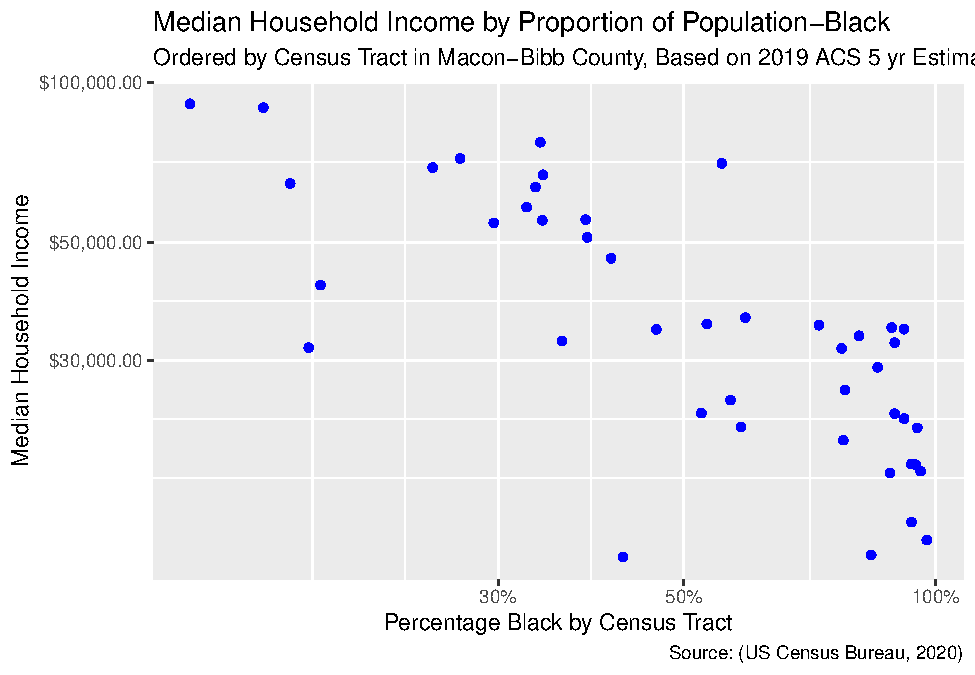
\includegraphics{UP494FinalProjectSubmission_Finkelstein_files/figure-latex/unnamed-chunk-7-1.pdf}

With the exception of one tract, which contains Mercer University and
benefits from the Census' counting of students as low income
individuals, every other tract in the low income category
(\textless\$30,000 for this context) is majority black. The highest
income tract, 134.10, is only 12\% black. It has a median household
income of \$91,116. Only one majority-black tract, 136.05, out of the 25
that are over half black has a median household income over \$40,000.
Its median household income is \$70,379. This demonstrates a high level
of inequality and presumed segregation, a consistent characteristic in
majority-minority communities.

A longitudinal comparison of the median household incomes in Tracts 101,
104, and 138 is tabulated with the following code:

\begin{Shaded}
\begin{Highlighting}[]
\NormalTok{areasmhi19 }\OtherTok{\textless{}{-}} \FunctionTok{get\_acs}\NormalTok{(}\AttributeTok{geography =} \StringTok{"tract"}\NormalTok{, }\AttributeTok{state =} \StringTok{"GA"}\NormalTok{, }\AttributeTok{county =} \StringTok{"Bibb"}\NormalTok{, }\AttributeTok{table =} \StringTok{"B19013"}\NormalTok{, }\AttributeTok{year=}\DecValTok{2019}\NormalTok{, }\AttributeTok{survey=}\StringTok{"acs5"}\NormalTok{, }\AttributeTok{output=}\StringTok{"wide"}\NormalTok{)}\SpecialCharTok{\%\textgreater{}\%}
\FunctionTok{filter}\NormalTok{(NAME }\SpecialCharTok{\%in\%} \FunctionTok{c}\NormalTok{(}\StringTok{"Census Tract 101, Bibb County, Georgia"}\NormalTok{, }\StringTok{"Census Tract 104, Bibb County, Georgia"}\NormalTok{, }\StringTok{"Census Tract 102, Bibb County, Georgia"}\NormalTok{)) }\SpecialCharTok{\%\textgreater{}\%}
\FunctionTok{mutate}\NormalTok{(}\AttributeTok{year =} \FunctionTok{case\_when}\NormalTok{(}
\NormalTok{  B19013\_001M }\SpecialCharTok{==} \StringTok{"8942"} \SpecialCharTok{\textasciitilde{}} \StringTok{"2019"}\NormalTok{,}
\NormalTok{  B19013\_001M }\SpecialCharTok{==} \StringTok{"4274"} \SpecialCharTok{\textasciitilde{}} \StringTok{"2019"}\NormalTok{,}
\NormalTok{  B19013\_001M }\SpecialCharTok{==} \StringTok{"7694"} \SpecialCharTok{\textasciitilde{}} \StringTok{"2019"}\NormalTok{) ) }\SpecialCharTok{\%\textgreater{}\%}
\FunctionTok{select}\NormalTok{(NAME, B19013\_001E, year) }\SpecialCharTok{\%\textgreater{}\%}
\FunctionTok{rename}\NormalTok{(}\AttributeTok{neighborhood =}\NormalTok{ NAME, }\AttributeTok{mhi =}\NormalTok{ B19013\_001E) }
\end{Highlighting}
\end{Shaded}

\begin{verbatim}
## Getting data from the 2015-2019 5-year ACS
\end{verbatim}

\begin{verbatim}
## Loading ACS5 variables for 2019 from table B19013. To cache this dataset for faster access to ACS tables in the future, run this function with `cache_table = TRUE`. You only need to do this once per ACS dataset.
\end{verbatim}

\begin{Shaded}
\begin{Highlighting}[]
\NormalTok{areasmhi18 }\OtherTok{\textless{}{-}} \FunctionTok{get\_acs}\NormalTok{(}\AttributeTok{geography =} \StringTok{"tract"}\NormalTok{, }\AttributeTok{state =} \StringTok{"GA"}\NormalTok{, }\AttributeTok{county =} \StringTok{"Bibb"}\NormalTok{, }\AttributeTok{table =} \StringTok{"B19013"}\NormalTok{, }\AttributeTok{year=}\DecValTok{2018}\NormalTok{, }\AttributeTok{survey=}\StringTok{"acs5"}\NormalTok{, }\AttributeTok{output=}\StringTok{"wide"}\NormalTok{)}\SpecialCharTok{\%\textgreater{}\%}
\FunctionTok{filter}\NormalTok{(NAME }\SpecialCharTok{\%in\%} \FunctionTok{c}\NormalTok{(}\StringTok{"Census Tract 102, Bibb County, Georgia"}\NormalTok{, }\StringTok{"Census Tract 104, Bibb County, Georgia"}\NormalTok{, }\StringTok{"Census Tract 101, Bibb County, Georgia"}\NormalTok{)) }\SpecialCharTok{\%\textgreater{}\%}
\FunctionTok{mutate}\NormalTok{(}\AttributeTok{year =} \FunctionTok{case\_when}\NormalTok{(}
\NormalTok{  B19013\_001M }\SpecialCharTok{==} \StringTok{"9704"} \SpecialCharTok{\textasciitilde{}} \StringTok{"2018"}\NormalTok{,}
\NormalTok{  B19013\_001M }\SpecialCharTok{==} \StringTok{"6460"} \SpecialCharTok{\textasciitilde{}} \StringTok{"2018"}\NormalTok{,}
\NormalTok{  B19013\_001M }\SpecialCharTok{==} \StringTok{"8050"} \SpecialCharTok{\textasciitilde{}} \StringTok{"2018"}\NormalTok{) ) }\SpecialCharTok{\%\textgreater{}\%}
\FunctionTok{select}\NormalTok{(NAME, B19013\_001E, year) }\SpecialCharTok{\%\textgreater{}\%}
\FunctionTok{rename}\NormalTok{(}\AttributeTok{neighborhood =}\NormalTok{ NAME, }\AttributeTok{mhi =}\NormalTok{ B19013\_001E) }
\end{Highlighting}
\end{Shaded}

\begin{verbatim}
## Getting data from the 2014-2018 5-year ACS
\end{verbatim}

\begin{verbatim}
## Loading ACS5 variables for 2018 from table B19013. To cache this dataset for faster access to ACS tables in the future, run this function with `cache_table = TRUE`. You only need to do this once per ACS dataset.
\end{verbatim}

\begin{Shaded}
\begin{Highlighting}[]
\NormalTok{areasmhi17 }\OtherTok{\textless{}{-}} \FunctionTok{get\_acs}\NormalTok{(}\AttributeTok{geography =} \StringTok{"tract"}\NormalTok{, }\AttributeTok{state =} \StringTok{"GA"}\NormalTok{, }\AttributeTok{county =} \StringTok{"Bibb"}\NormalTok{, }\AttributeTok{table =} \StringTok{"B19013"}\NormalTok{, }\AttributeTok{year=}\DecValTok{2017}\NormalTok{, }\AttributeTok{survey=}\StringTok{"acs5"}\NormalTok{, }\AttributeTok{output=}\StringTok{"wide"}\NormalTok{) }\SpecialCharTok{\%\textgreater{}\%}
\FunctionTok{filter}\NormalTok{(NAME }\SpecialCharTok{\%in\%} \FunctionTok{c}\NormalTok{(}\StringTok{"Census Tract 101, Bibb County, Georgia"}\NormalTok{, }\StringTok{"Census Tract 104, Bibb County, Georgia"}\NormalTok{, }\StringTok{"Census Tract 102, Bibb County, Georgia"}\NormalTok{)) }\SpecialCharTok{\%\textgreater{}\%}
\FunctionTok{mutate}\NormalTok{(}\AttributeTok{year =} \FunctionTok{case\_when}\NormalTok{(}
\NormalTok{  B19013\_001M }\SpecialCharTok{==} \StringTok{"5841"} \SpecialCharTok{\textasciitilde{}} \StringTok{"2017"}\NormalTok{,}
\NormalTok{  B19013\_001M }\SpecialCharTok{==} \StringTok{"7934"} \SpecialCharTok{\textasciitilde{}} \StringTok{"2017"}\NormalTok{,}
\NormalTok{  B19013\_001M }\SpecialCharTok{==} \StringTok{"5353"} \SpecialCharTok{\textasciitilde{}} \StringTok{"2017"}\NormalTok{) ) }\SpecialCharTok{\%\textgreater{}\%}
\FunctionTok{select}\NormalTok{(NAME, B19013\_001E, year) }\SpecialCharTok{\%\textgreater{}\%}
\FunctionTok{rename}\NormalTok{(}\AttributeTok{neighborhood =}\NormalTok{ NAME, }\AttributeTok{mhi =}\NormalTok{ B19013\_001E)}
\end{Highlighting}
\end{Shaded}

\begin{verbatim}
## Getting data from the 2013-2017 5-year ACS
\end{verbatim}

\begin{verbatim}
## Loading ACS5 variables for 2017 from table B19013. To cache this dataset for faster access to ACS tables in the future, run this function with `cache_table = TRUE`. You only need to do this once per ACS dataset.
\end{verbatim}

\begin{Shaded}
\begin{Highlighting}[]
\NormalTok{areasmhi16 }\OtherTok{\textless{}{-}} \FunctionTok{get\_acs}\NormalTok{(}\AttributeTok{geography =} \StringTok{"tract"}\NormalTok{, }\AttributeTok{state =} \StringTok{"GA"}\NormalTok{, }\AttributeTok{county =} \StringTok{"Bibb"}\NormalTok{, }\AttributeTok{table =} \StringTok{"B19013"}\NormalTok{, }\AttributeTok{year=}\DecValTok{2016}\NormalTok{, }\AttributeTok{survey=}\StringTok{"acs5"}\NormalTok{, }\AttributeTok{output=}\StringTok{"wide"}\NormalTok{) }\SpecialCharTok{\%\textgreater{}\%}
\FunctionTok{filter}\NormalTok{(NAME }\SpecialCharTok{\%in\%} \FunctionTok{c}\NormalTok{(}\StringTok{"Census Tract 101, Bibb County, Georgia"}\NormalTok{, }\StringTok{"Census Tract 104, Bibb County, Georgia"}\NormalTok{, }\StringTok{"Census Tract 102, Bibb County, Georgia"}\NormalTok{)) }\SpecialCharTok{\%\textgreater{}\%}
\FunctionTok{mutate}\NormalTok{(}\AttributeTok{year =} \FunctionTok{case\_when}\NormalTok{(}
\NormalTok{  B19013\_001M }\SpecialCharTok{==} \StringTok{"5466"} \SpecialCharTok{\textasciitilde{}} \StringTok{"2016"}\NormalTok{,}
\NormalTok{  B19013\_001M }\SpecialCharTok{==} \StringTok{"8125"} \SpecialCharTok{\textasciitilde{}} \StringTok{"2016"}\NormalTok{,}
\NormalTok{  B19013\_001M }\SpecialCharTok{==} \StringTok{"3078"} \SpecialCharTok{\textasciitilde{}} \StringTok{"2016"}\NormalTok{) ) }\SpecialCharTok{\%\textgreater{}\%}
\FunctionTok{select}\NormalTok{(NAME, B19013\_001E, year) }\SpecialCharTok{\%\textgreater{}\%}
\FunctionTok{rename}\NormalTok{(}\AttributeTok{neighborhood =}\NormalTok{ NAME, }\AttributeTok{mhi =}\NormalTok{ B19013\_001E)}
\end{Highlighting}
\end{Shaded}

\begin{verbatim}
## Getting data from the 2012-2016 5-year ACS
\end{verbatim}

\begin{verbatim}
## Loading ACS5 variables for 2016 from table B19013. To cache this dataset for faster access to ACS tables in the future, run this function with `cache_table = TRUE`. You only need to do this once per ACS dataset.
\end{verbatim}

\begin{Shaded}
\begin{Highlighting}[]
\NormalTok{areasmhi15 }\OtherTok{\textless{}{-}} \FunctionTok{get\_acs}\NormalTok{(}\AttributeTok{geography =} \StringTok{"tract"}\NormalTok{, }\AttributeTok{state =} \StringTok{"GA"}\NormalTok{, }\AttributeTok{county =} \StringTok{"Bibb"}\NormalTok{, }\AttributeTok{table =} \StringTok{"B19013"}\NormalTok{, }\AttributeTok{year=}\DecValTok{2015}\NormalTok{, }\AttributeTok{survey=}\StringTok{"acs5"}\NormalTok{, }\AttributeTok{output=}\StringTok{"wide"}\NormalTok{) }\SpecialCharTok{\%\textgreater{}\%}
\FunctionTok{filter}\NormalTok{(NAME }\SpecialCharTok{\%in\%} \FunctionTok{c}\NormalTok{(}\StringTok{"Census Tract 101, Bibb County, Georgia"}\NormalTok{, }\StringTok{"Census Tract 104, Bibb County, Georgia"}\NormalTok{, }\StringTok{"Census Tract 102, Bibb County, Georgia"}\NormalTok{)) }\SpecialCharTok{\%\textgreater{}\%}
\FunctionTok{mutate}\NormalTok{(}\AttributeTok{year =} \FunctionTok{case\_when}\NormalTok{(}
\NormalTok{  B19013\_001M }\SpecialCharTok{==} \StringTok{"4240"} \SpecialCharTok{\textasciitilde{}} \StringTok{"2015"}\NormalTok{,}
\NormalTok{  B19013\_001M }\SpecialCharTok{==} \StringTok{"2629"} \SpecialCharTok{\textasciitilde{}} \StringTok{"2015"}\NormalTok{,}
\NormalTok{  B19013\_001M }\SpecialCharTok{==} \StringTok{"4138"} \SpecialCharTok{\textasciitilde{}} \StringTok{"2015"}\NormalTok{) ) }\SpecialCharTok{\%\textgreater{}\%}
\FunctionTok{select}\NormalTok{(NAME, B19013\_001E, year) }\SpecialCharTok{\%\textgreater{}\%}
\FunctionTok{rename}\NormalTok{(}\AttributeTok{neighborhood =}\NormalTok{ NAME, }\AttributeTok{mhi =}\NormalTok{ B19013\_001E) }
\end{Highlighting}
\end{Shaded}

\begin{verbatim}
## Getting data from the 2011-2015 5-year ACS
\end{verbatim}

\begin{verbatim}
## Loading ACS5 variables for 2015 from table B19013. To cache this dataset for faster access to ACS tables in the future, run this function with `cache_table = TRUE`. You only need to do this once per ACS dataset.
\end{verbatim}

\begin{Shaded}
\begin{Highlighting}[]
\NormalTok{areas5yr}\OtherTok{\textless{}{-}} \FunctionTok{bind\_rows}\NormalTok{(areasmhi15, areasmhi16, areasmhi17, areasmhi18, areasmhi19) }
\end{Highlighting}
\end{Shaded}

And here is the accompanying line graph for the table

\begin{Shaded}
\begin{Highlighting}[]
\NormalTok{lastfivemhi }\OtherTok{\textless{}{-}} \FunctionTok{ggplot}\NormalTok{(areas5yr, }\FunctionTok{aes}\NormalTok{(}\AttributeTok{x =}\NormalTok{ year, }\AttributeTok{y =}\NormalTok{ mhi, }\AttributeTok{group =}\NormalTok{ neighborhood)) }\SpecialCharTok{+} 
\FunctionTok{geom\_line}\NormalTok{(}\FunctionTok{aes}\NormalTok{(}\AttributeTok{color=}\NormalTok{neighborhood)) }\SpecialCharTok{+}
\FunctionTok{geom\_point}\NormalTok{(}\FunctionTok{aes}\NormalTok{(}\AttributeTok{color=}\NormalTok{neighborhood)) }\SpecialCharTok{+}
\FunctionTok{scale\_y\_log10}\NormalTok{(}\AttributeTok{labels=}\NormalTok{scales}\SpecialCharTok{::}\NormalTok{dollar)}\SpecialCharTok{+}
\FunctionTok{labs}\NormalTok{(}\AttributeTok{x =} \StringTok{"Year"}\NormalTok{, }\AttributeTok{y =} \StringTok{"Median Household Income"}\NormalTok{,}
     \AttributeTok{title =} \StringTok{"Median Household Income in Three Comparison Neighborhoods by Year"}\NormalTok{,}
     \AttributeTok{caption =} \StringTok{"Source: (US Census Bureau: 2016{-}2020)"}\NormalTok{)}
\end{Highlighting}
\end{Shaded}

\begin{Shaded}
\begin{Highlighting}[]
\NormalTok{areas5yr}
\end{Highlighting}
\end{Shaded}

\begin{verbatim}
## # A tibble: 15 x 3
##    neighborhood                             mhi year 
##    <chr>                                  <dbl> <chr>
##  1 Census Tract 101, Bibb County, Georgia 13097 2015 
##  2 Census Tract 104, Bibb County, Georgia 12962 2015 
##  3 Census Tract 102, Bibb County, Georgia 25080 2015 
##  4 Census Tract 101, Bibb County, Georgia 17708 2016 
##  5 Census Tract 104, Bibb County, Georgia 17031 2016 
##  6 Census Tract 102, Bibb County, Georgia 26191 2016 
##  7 Census Tract 101, Bibb County, Georgia 18333 2017 
##  8 Census Tract 104, Bibb County, Georgia 19018 2017 
##  9 Census Tract 102, Bibb County, Georgia 31162 2017 
## 10 Census Tract 101, Bibb County, Georgia 21902 2018 
## 11 Census Tract 104, Bibb County, Georgia 22500 2018 
## 12 Census Tract 102, Bibb County, Georgia 35373 2018 
## 13 Census Tract 101, Bibb County, Georgia 18542 2019 
## 14 Census Tract 104, Bibb County, Georgia 23281 2019 
## 15 Census Tract 102, Bibb County, Georgia 32578 2019
\end{verbatim}

\begin{Shaded}
\begin{Highlighting}[]
\NormalTok{lastfivemhi}
\end{Highlighting}
\end{Shaded}

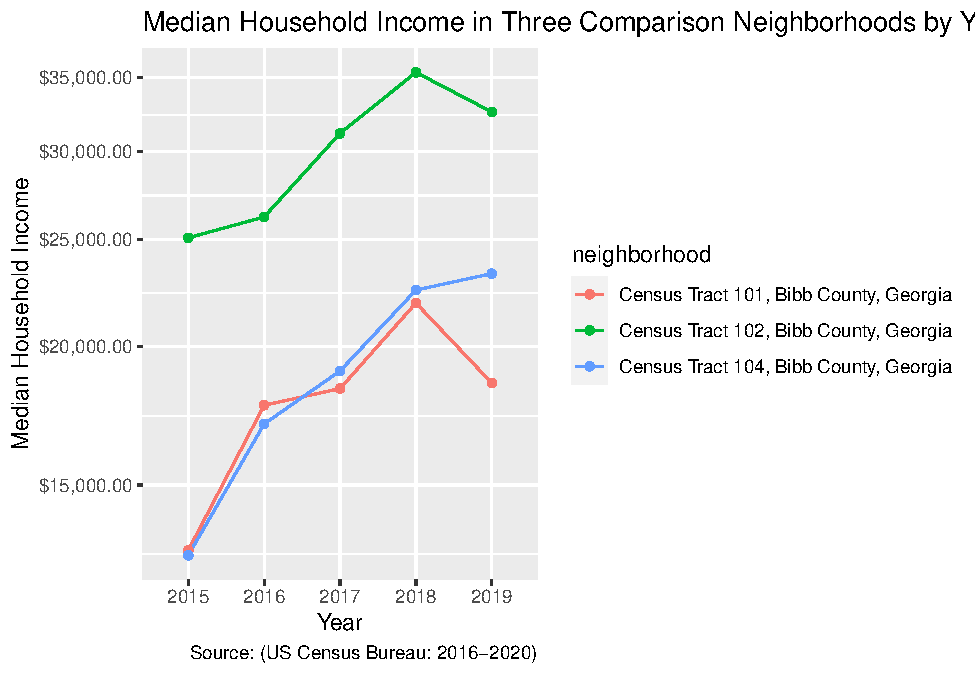
\includegraphics{UP494FinalProjectSubmission_Finkelstein_files/figure-latex/unnamed-chunk-11-1.pdf}

According to analysis, Unionville actually experienced a most consistent
increase in median household income. However, it is unclear if this is
indication of increasing prosperity or further property investment for
rental properties. A five year sample may also not provide the strongest
indication of changes in area income. Another indicator surrounding
housing utilization may give a stronger indication of general changes in
prosperity and neighborhood health.

A longitudinal comparison of the occupancy rates in Tracts 101, 104, and
138 is tabulated with the following code:

\begin{Shaded}
\begin{Highlighting}[]
\NormalTok{vacancyrate19 }\OtherTok{\textless{}{-}} \FunctionTok{get\_acs}\NormalTok{(}\AttributeTok{geography =} \StringTok{"tract"}\NormalTok{, }\AttributeTok{state =} \StringTok{"GA"}\NormalTok{, }\AttributeTok{county =} \StringTok{"Bibb"}\NormalTok{, }\AttributeTok{table =} \StringTok{"DP04"}\NormalTok{,  }\AttributeTok{year=}\DecValTok{2019}\NormalTok{, }\AttributeTok{survey=}\StringTok{"acs5"}\NormalTok{, }\AttributeTok{output=}\StringTok{"wide"}\NormalTok{)}\SpecialCharTok{\%\textgreater{}\%}
\FunctionTok{filter}\NormalTok{(NAME }\SpecialCharTok{\%in\%} \FunctionTok{c}\NormalTok{(}\StringTok{"Census Tract 101, Bibb County, Georgia"}\NormalTok{, }\StringTok{"Census Tract 104, Bibb County, Georgia"}\NormalTok{, }\StringTok{"Census Tract 102, Bibb County, Georgia"}\NormalTok{)) }\SpecialCharTok{\%\textgreater{}\%}
  \FunctionTok{mutate}\NormalTok{(}\AttributeTok{year =} \FunctionTok{case\_when}\NormalTok{(}
\NormalTok{    DP04\_0003PM }\SpecialCharTok{==} \StringTok{"9.8"} \SpecialCharTok{\textasciitilde{}} \StringTok{"2019"}\NormalTok{,}
\NormalTok{    DP04\_0003PM }\SpecialCharTok{==} \StringTok{"8.3"} \SpecialCharTok{\textasciitilde{}} \StringTok{"2019"}\NormalTok{,}
\NormalTok{    DP04\_0003PM }\SpecialCharTok{==} \StringTok{"7.1"} \SpecialCharTok{\textasciitilde{}} \StringTok{"2019"}
\NormalTok{  )) }\SpecialCharTok{\%\textgreater{}\%}
  \FunctionTok{rename}\NormalTok{(}\AttributeTok{Neighborhood =}\NormalTok{ NAME,}
         \AttributeTok{Properties =}\NormalTok{ DP04\_0001E,}
         \AttributeTok{Occupied =}\NormalTok{ DP04\_0002E,}
         \AttributeTok{Percent\_Occupied =}\NormalTok{ DP04\_0002PE,}
         \AttributeTok{Percent\_Vacant =}\NormalTok{ DP04\_0003PE) }\SpecialCharTok{\%\textgreater{}\%}
   \FunctionTok{select}\NormalTok{(Neighborhood, Properties, Occupied, Percent\_Occupied, Percent\_Vacant, year) }
\end{Highlighting}
\end{Shaded}

\begin{verbatim}
## Getting data from the 2015-2019 5-year ACS
\end{verbatim}

\begin{verbatim}
## Loading ACS5/PROFILE variables for 2019 from table DP04. To cache this dataset for faster access to ACS tables in the future, run this function with `cache_table = TRUE`. You only need to do this once per ACS dataset.
\end{verbatim}

\begin{verbatim}
## Using the ACS Data Profile
## Using the ACS Data Profile
## Using the ACS Data Profile
## Using the ACS Data Profile
## Using the ACS Data Profile
## Using the ACS Data Profile
## Using the ACS Data Profile
## Using the ACS Data Profile
## Using the ACS Data Profile
## Using the ACS Data Profile
## Using the ACS Data Profile
## Using the ACS Data Profile
\end{verbatim}

\begin{Shaded}
\begin{Highlighting}[]
\NormalTok{vacancyrate18 }\OtherTok{\textless{}{-}} \FunctionTok{get\_acs}\NormalTok{(}\AttributeTok{geography =} \StringTok{"tract"}\NormalTok{, }\AttributeTok{state =} \StringTok{"GA"}\NormalTok{, }\AttributeTok{county =} \StringTok{"Bibb"}\NormalTok{, }\AttributeTok{table =} \StringTok{"DP04"}\NormalTok{,  }\AttributeTok{year=}\DecValTok{2018}\NormalTok{, }\AttributeTok{survey=}\StringTok{"acs5"}\NormalTok{, }\AttributeTok{output=}\StringTok{"wide"}\NormalTok{)}\SpecialCharTok{\%\textgreater{}\%}
\FunctionTok{filter}\NormalTok{(NAME }\SpecialCharTok{\%in\%} \FunctionTok{c}\NormalTok{(}\StringTok{"Census Tract 101, Bibb County, Georgia"}\NormalTok{, }\StringTok{"Census Tract 104, Bibb County, Georgia"}\NormalTok{, }\StringTok{"Census Tract 102, Bibb County, Georgia"}\NormalTok{)) }\SpecialCharTok{\%\textgreater{}\%}
  \FunctionTok{mutate}\NormalTok{(}\AttributeTok{year =} \FunctionTok{case\_when}\NormalTok{(}
\NormalTok{    DP04\_0003PM }\SpecialCharTok{==} \StringTok{"6.9"} \SpecialCharTok{\textasciitilde{}} \StringTok{"2018"}\NormalTok{,}
\NormalTok{    DP04\_0003PM }\SpecialCharTok{==} \StringTok{"8.3"} \SpecialCharTok{\textasciitilde{}} \StringTok{"2018"}\NormalTok{,}
\NormalTok{    DP04\_0003PM }\SpecialCharTok{==} \StringTok{"7.7"} \SpecialCharTok{\textasciitilde{}} \StringTok{"2018"}
\NormalTok{  )) }\SpecialCharTok{\%\textgreater{}\%}
  \FunctionTok{rename}\NormalTok{(}\AttributeTok{Neighborhood =}\NormalTok{ NAME,}
         \AttributeTok{Properties =}\NormalTok{ DP04\_0001E,}
         \AttributeTok{Occupied =}\NormalTok{ DP04\_0002E,}
         \AttributeTok{Percent\_Occupied =}\NormalTok{ DP04\_0002PE,}
         \AttributeTok{Percent\_Vacant =}\NormalTok{ DP04\_0003PE) }\SpecialCharTok{\%\textgreater{}\%}
   \FunctionTok{select}\NormalTok{(Neighborhood, Properties, Occupied, Percent\_Occupied, Percent\_Vacant, year) }
\end{Highlighting}
\end{Shaded}

\begin{verbatim}
## Getting data from the 2014-2018 5-year ACS
\end{verbatim}

\begin{verbatim}
## Loading ACS5/PROFILE variables for 2018 from table DP04. To cache this dataset for faster access to ACS tables in the future, run this function with `cache_table = TRUE`. You only need to do this once per ACS dataset.
\end{verbatim}

\begin{verbatim}
## Using the ACS Data Profile
## Using the ACS Data Profile
## Using the ACS Data Profile
## Using the ACS Data Profile
## Using the ACS Data Profile
## Using the ACS Data Profile
## Using the ACS Data Profile
## Using the ACS Data Profile
## Using the ACS Data Profile
## Using the ACS Data Profile
## Using the ACS Data Profile
## Using the ACS Data Profile
\end{verbatim}

\begin{Shaded}
\begin{Highlighting}[]
\NormalTok{vacancyrate17 }\OtherTok{\textless{}{-}} \FunctionTok{get\_acs}\NormalTok{(}\AttributeTok{geography =} \StringTok{"tract"}\NormalTok{, }\AttributeTok{state =} \StringTok{"GA"}\NormalTok{, }\AttributeTok{county =} \StringTok{"Bibb"}\NormalTok{, }\AttributeTok{table =} \StringTok{"DP04"}\NormalTok{,  }\AttributeTok{year=}\DecValTok{2017}\NormalTok{, }\AttributeTok{survey=}\StringTok{"acs5"}\NormalTok{, }\AttributeTok{output=}\StringTok{"wide"}\NormalTok{)}\SpecialCharTok{\%\textgreater{}\%}
\FunctionTok{filter}\NormalTok{(NAME }\SpecialCharTok{\%in\%} \FunctionTok{c}\NormalTok{(}\StringTok{"Census Tract 101, Bibb County, Georgia"}\NormalTok{, }\StringTok{"Census Tract 104, Bibb County, Georgia"}\NormalTok{, }\StringTok{"Census Tract 102, Bibb County, Georgia"}\NormalTok{)) }\SpecialCharTok{\%\textgreater{}\%}
  \FunctionTok{mutate}\NormalTok{(}\AttributeTok{year =} \FunctionTok{case\_when}\NormalTok{(}
\NormalTok{    DP04\_0003PM }\SpecialCharTok{==} \StringTok{"8.4"} \SpecialCharTok{\textasciitilde{}} \StringTok{"2017"}\NormalTok{,}
\NormalTok{    DP04\_0003PM }\SpecialCharTok{==} \StringTok{"7.4"} \SpecialCharTok{\textasciitilde{}} \StringTok{"2017"}\NormalTok{,}
\NormalTok{    DP04\_0003PM }\SpecialCharTok{==} \StringTok{"8.9"} \SpecialCharTok{\textasciitilde{}} \StringTok{"2017"}
\NormalTok{  )) }\SpecialCharTok{\%\textgreater{}\%}
  \FunctionTok{rename}\NormalTok{(}\AttributeTok{Neighborhood =}\NormalTok{ NAME,}
         \AttributeTok{Properties =}\NormalTok{ DP04\_0001E,}
         \AttributeTok{Occupied =}\NormalTok{ DP04\_0002E,}
         \AttributeTok{Percent\_Occupied =}\NormalTok{ DP04\_0002PE,}
         \AttributeTok{Percent\_Vacant =}\NormalTok{ DP04\_0003PE) }\SpecialCharTok{\%\textgreater{}\%}
   \FunctionTok{select}\NormalTok{(Neighborhood, Properties, Occupied, Percent\_Occupied, Percent\_Vacant, year) }
\end{Highlighting}
\end{Shaded}

\begin{verbatim}
## Getting data from the 2013-2017 5-year ACS
\end{verbatim}

\begin{verbatim}
## Loading ACS5/PROFILE variables for 2017 from table DP04. To cache this dataset for faster access to ACS tables in the future, run this function with `cache_table = TRUE`. You only need to do this once per ACS dataset.
\end{verbatim}

\begin{verbatim}
## Using the ACS Data Profile
## Using the ACS Data Profile
## Using the ACS Data Profile
## Using the ACS Data Profile
## Using the ACS Data Profile
## Using the ACS Data Profile
## Using the ACS Data Profile
## Using the ACS Data Profile
## Using the ACS Data Profile
## Using the ACS Data Profile
## Using the ACS Data Profile
## Using the ACS Data Profile
\end{verbatim}

\begin{Shaded}
\begin{Highlighting}[]
\NormalTok{vacancyrate16 }\OtherTok{\textless{}{-}} \FunctionTok{get\_acs}\NormalTok{(}\AttributeTok{geography =} \StringTok{"tract"}\NormalTok{, }\AttributeTok{state =} \StringTok{"GA"}\NormalTok{, }\AttributeTok{county =} \StringTok{"Bibb"}\NormalTok{, }\AttributeTok{table =} \StringTok{"DP04"}\NormalTok{,  }\AttributeTok{year=}\DecValTok{2016}\NormalTok{, }\AttributeTok{survey=}\StringTok{"acs5"}\NormalTok{, }\AttributeTok{output=}\StringTok{"wide"}\NormalTok{)}\SpecialCharTok{\%\textgreater{}\%}
\FunctionTok{filter}\NormalTok{(NAME }\SpecialCharTok{\%in\%} \FunctionTok{c}\NormalTok{(}\StringTok{"Census Tract 101, Bibb County, Georgia"}\NormalTok{, }\StringTok{"Census Tract 104, Bibb County, Georgia"}\NormalTok{, }\StringTok{"Census Tract 102, Bibb County, Georgia"}\NormalTok{)) }\SpecialCharTok{\%\textgreater{}\%}
  \FunctionTok{mutate}\NormalTok{(}\AttributeTok{year =} \FunctionTok{case\_when}\NormalTok{(}
\NormalTok{    DP04\_0003PE }\SpecialCharTok{==} \StringTok{"18.9"} \SpecialCharTok{\textasciitilde{}} \StringTok{"2016"}\NormalTok{,}
\NormalTok{    DP04\_0003PE }\SpecialCharTok{==} \StringTok{"34.1"} \SpecialCharTok{\textasciitilde{}} \StringTok{"2016"}\NormalTok{,}
\NormalTok{    DP04\_0003PE }\SpecialCharTok{==} \StringTok{"43.5"} \SpecialCharTok{\textasciitilde{}} \StringTok{"2016"}
\NormalTok{  )) }\SpecialCharTok{\%\textgreater{}\%}
  \FunctionTok{rename}\NormalTok{(}\AttributeTok{Neighborhood =}\NormalTok{ NAME,}
         \AttributeTok{Properties =}\NormalTok{ DP04\_0001E,}
         \AttributeTok{Occupied =}\NormalTok{ DP04\_0002E,}
         \AttributeTok{Percent\_Occupied =}\NormalTok{ DP04\_0002PE,}
         \AttributeTok{Percent\_Vacant =}\NormalTok{ DP04\_0003PE) }\SpecialCharTok{\%\textgreater{}\%}
   \FunctionTok{select}\NormalTok{(Neighborhood, Properties, Occupied, Percent\_Occupied, Percent\_Vacant, year) }
\end{Highlighting}
\end{Shaded}

\begin{verbatim}
## Getting data from the 2012-2016 5-year ACS
\end{verbatim}

\begin{verbatim}
## Loading ACS5/PROFILE variables for 2016 from table DP04. To cache this dataset for faster access to ACS tables in the future, run this function with `cache_table = TRUE`. You only need to do this once per ACS dataset.
\end{verbatim}

\begin{verbatim}
## Using the ACS Data Profile
## Using the ACS Data Profile
## Using the ACS Data Profile
## Using the ACS Data Profile
## Using the ACS Data Profile
## Using the ACS Data Profile
## Using the ACS Data Profile
## Using the ACS Data Profile
## Using the ACS Data Profile
## Using the ACS Data Profile
## Using the ACS Data Profile
## Using the ACS Data Profile
\end{verbatim}

\begin{Shaded}
\begin{Highlighting}[]
\NormalTok{vacancyrate15 }\OtherTok{\textless{}{-}} \FunctionTok{get\_acs}\NormalTok{(}\AttributeTok{geography =} \StringTok{"tract"}\NormalTok{, }\AttributeTok{state =} \StringTok{"GA"}\NormalTok{, }\AttributeTok{county =} \StringTok{"Bibb"}\NormalTok{, }\AttributeTok{table =} \StringTok{"DP04"}\NormalTok{,  }\AttributeTok{year=}\DecValTok{2015}\NormalTok{, }\AttributeTok{survey=}\StringTok{"acs5"}\NormalTok{, }\AttributeTok{output=}\StringTok{"wide"}\NormalTok{)}\SpecialCharTok{\%\textgreater{}\%}
\FunctionTok{filter}\NormalTok{(NAME }\SpecialCharTok{\%in\%} \FunctionTok{c}\NormalTok{(}\StringTok{"Census Tract 101, Bibb County, Georgia"}\NormalTok{, }\StringTok{"Census Tract 104, Bibb County, Georgia"}\NormalTok{, }\StringTok{"Census Tract 102, Bibb County, Georgia"}\NormalTok{)) }\SpecialCharTok{\%\textgreater{}\%}
  \FunctionTok{mutate}\NormalTok{(}\AttributeTok{year =} \FunctionTok{case\_when}\NormalTok{(}
\NormalTok{    DP04\_0003PM }\SpecialCharTok{==} \StringTok{"7.3"} \SpecialCharTok{\textasciitilde{}} \StringTok{"2015"}\NormalTok{,}
\NormalTok{    DP04\_0003PM }\SpecialCharTok{==} \StringTok{"7.8"} \SpecialCharTok{\textasciitilde{}} \StringTok{"2015"}\NormalTok{,}
\NormalTok{    DP04\_0003PM }\SpecialCharTok{==} \StringTok{"8.4"} \SpecialCharTok{\textasciitilde{}} \StringTok{"2015"}
\NormalTok{  )) }\SpecialCharTok{\%\textgreater{}\%}
  \FunctionTok{rename}\NormalTok{(}\AttributeTok{Neighborhood =}\NormalTok{ NAME,}
         \AttributeTok{Properties =}\NormalTok{ DP04\_0001E,}
         \AttributeTok{Occupied =}\NormalTok{ DP04\_0002E,}
         \AttributeTok{Percent\_Occupied =}\NormalTok{ DP04\_0002PE,}
         \AttributeTok{Percent\_Vacant =}\NormalTok{ DP04\_0003PE) }\SpecialCharTok{\%\textgreater{}\%}
   \FunctionTok{select}\NormalTok{(Neighborhood, Properties, Occupied, Percent\_Occupied, Percent\_Vacant, year) }
\end{Highlighting}
\end{Shaded}

\begin{verbatim}
## Getting data from the 2011-2015 5-year ACS
\end{verbatim}

\begin{verbatim}
## Loading ACS5/PROFILE variables for 2015 from table DP04. To cache this dataset for faster access to ACS tables in the future, run this function with `cache_table = TRUE`. You only need to do this once per ACS dataset.
\end{verbatim}

\begin{verbatim}
## Using the ACS Data Profile
## Using the ACS Data Profile
## Using the ACS Data Profile
## Using the ACS Data Profile
## Using the ACS Data Profile
## Using the ACS Data Profile
## Using the ACS Data Profile
## Using the ACS Data Profile
## Using the ACS Data Profile
## Using the ACS Data Profile
## Using the ACS Data Profile
## Using the ACS Data Profile
\end{verbatim}

\begin{Shaded}
\begin{Highlighting}[]
\NormalTok{vacancyrates5yr }\OtherTok{\textless{}{-}} \FunctionTok{bind\_rows}\NormalTok{(vacancyrate15, vacancyrate16, vacancyrate17, vacancyrate18, vacancyrate19)}
\end{Highlighting}
\end{Shaded}

The following graph shows the change in vacancy rate over time:

\begin{Shaded}
\begin{Highlighting}[]
\NormalTok{lastfivevacancy }\OtherTok{\textless{}{-}} \FunctionTok{ggplot}\NormalTok{(vacancyrates5yr, }\FunctionTok{aes}\NormalTok{(}\AttributeTok{x =}\NormalTok{ year, }\AttributeTok{y =}\NormalTok{ Percent\_Vacant, }\AttributeTok{group =}\NormalTok{ Neighborhood)) }\SpecialCharTok{+} 
\FunctionTok{geom\_line}\NormalTok{(}\FunctionTok{aes}\NormalTok{(}\AttributeTok{color=}\NormalTok{Neighborhood)) }\SpecialCharTok{+}
\FunctionTok{geom\_point}\NormalTok{(}\FunctionTok{aes}\NormalTok{(}\AttributeTok{color=}\NormalTok{Neighborhood)) }\SpecialCharTok{+}
\FunctionTok{labs}\NormalTok{(}\AttributeTok{x =} \StringTok{"Year"}\NormalTok{, }\AttributeTok{y =} \StringTok{"Vacancy Rate(\%)"}\NormalTok{,}
     \AttributeTok{title =} \StringTok{"Vacancy Rate in Three Comparison Neighborhoods by Year"}\NormalTok{,}
     \AttributeTok{caption =} \StringTok{"Source: (US Census Bureau: 2016{-}2020)"}\NormalTok{ )}
\end{Highlighting}
\end{Shaded}

\begin{Shaded}
\begin{Highlighting}[]
\NormalTok{vacancyrates5yr}
\end{Highlighting}
\end{Shaded}

\begin{verbatim}
## # A tibble: 15 x 6
##    Neighborhood        Properties Occupied Percent_Occupied Percent_Vacant year 
##    <chr>                    <dbl>    <dbl>            <dbl>          <dbl> <chr>
##  1 Census Tract 101, ~       1054      621             58.9           41.1 2015 
##  2 Census Tract 104, ~       1394      925             66.4           33.6 2015 
##  3 Census Tract 102, ~       1289     1013             78.6           21.4 2015 
##  4 Census Tract 101, ~       1067      603             56.5           43.5 2016 
##  5 Census Tract 104, ~       1328      875             65.9           34.1 2016 
##  6 Census Tract 102, ~       1309     1061             81.1           18.9 2016 
##  7 Census Tract 101, ~       1025      598             58.3           41.7 2017 
##  8 Census Tract 104, ~       1347      766             56.9           43.1 2017 
##  9 Census Tract 102, ~       1313     1026             78.1           21.9 2017 
## 10 Census Tract 101, ~        993      643             64.8           35.2 2018 
## 11 Census Tract 104, ~       1287      730             56.7           43.3 2018 
## 12 Census Tract 102, ~       1276      974             76.3           23.7 2018 
## 13 Census Tract 101, ~        953      632             66.3           33.7 2019 
## 14 Census Tract 104, ~       1259      726             57.7           42.3 2019 
## 15 Census Tract 102, ~       1325      962             72.6           27.4 2019
\end{verbatim}

\begin{Shaded}
\begin{Highlighting}[]
\NormalTok{lastfivevacancy}
\end{Highlighting}
\end{Shaded}

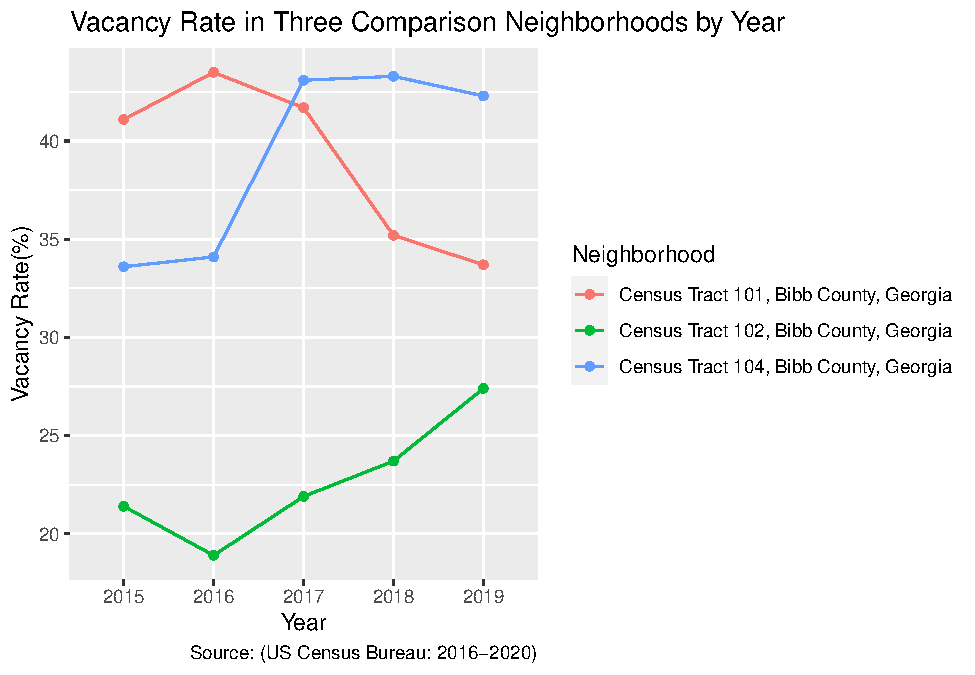
\includegraphics{UP494FinalProjectSubmission_Finkelstein_files/figure-latex/unnamed-chunk-15-1.pdf}

Admittedly, vacancy rate is an imperfect indication of blight. But
drastic declines in Pleasant Hill's vacancy rate. back up the
involvement of public strategies to eliminate blight, either for housing
rehabilitation or demolition to increase open space. These include a
growing blight bond project and an effort funded by the Georgia
Department of Transportation to relocate and rebuild homes demolished by
their Interstate 25 expansion. Census Tract 102, Vineville, has
increasing vacancy rate likely pertaining to incresed rental properties
and an increasing number of unoccupied, historic homes on the busy main
road. And Vineville still has around 30\% less of the vacancy that
Unionville has.

\begin{Shaded}
\begin{Highlighting}[]
\CommentTok{\#Loading}
\NormalTok{d5crime }\OtherTok{\textless{}{-}}\NormalTok{ (}\FunctionTok{read.csv}\NormalTok{(}\StringTok{"MACON{-}BIBB COMMMISION DISTRICT 5\_crime.csv"}\NormalTok{))}
\NormalTok{SCFd5}\OtherTok{\textless{}{-}}\NormalTok{(}\FunctionTok{read.csv}\NormalTok{(}\StringTok{"District 5 info\_seeclickfix.csv"}\NormalTok{))}
\NormalTok{MostImportantComplaints }\OtherTok{\textless{}{-}}\NormalTok{ (}\FunctionTok{read.csv}\NormalTok{(}\StringTok{"District 5 narroweddown\_seeclickfix.csv"}\NormalTok{))}
\end{Highlighting}
\end{Shaded}

\hypertarget{crime-in-district-5-and-select-neighborhoods}{%
\section{Crime In District 5 and Select
Neighborhoods}\label{crime-in-district-5-and-select-neighborhoods}}

This first hyper local comparison involves looking at the reported crime
rates for 2020 in each neighborhood as a percentage of the District 5
total. Below are a table and graph representing the following:

\begin{enumerate}
\def\labelenumi{\arabic{enumi}.}
\tightlist
\item
  Unionville, Pleasant Hill, and Vineville's percentages of the total
  crime rate for District 5
\item
  The proportion of each reported crime type to the whole in Unionville,
  Pleasant Hill, and Vineville
\item
  Streets and intersections in Unionville With Over Three Reported
  Events.
\end{enumerate}

First, here is the code pertaining to the crime tables and graphs:

\begin{Shaded}
\begin{Highlighting}[]
\NormalTok{d5crime }\OtherTok{\textless{}{-}}\NormalTok{ d5crime }\SpecialCharTok{\%\textgreater{}\%} 
  \FunctionTok{select}\NormalTok{(ï..Address, IncidentÂ.Type, Neighborhood) }\SpecialCharTok{\%\textgreater{}\%}
  \FunctionTok{rename}\NormalTok{(}\AttributeTok{Address =}\NormalTok{ ï..Address, }\AttributeTok{Type=}\NormalTok{ IncidentÂ.Type) }\SpecialCharTok{\%\textgreater{}\%} 
  \FunctionTok{mutate}\NormalTok{(}\AttributeTok{StreetName =} \FunctionTok{rm\_number}\NormalTok{(Address))}
   
\NormalTok{d5neighborhood }\OtherTok{\textless{}{-}}\NormalTok{ d5crime }\SpecialCharTok{\%\textgreater{}\%}
  \FunctionTok{filter}\NormalTok{(Neighborhood }\SpecialCharTok{\%in\%} \FunctionTok{c}\NormalTok{(}\StringTok{"U"}\NormalTok{, }\StringTok{"PH"}\NormalTok{, }\StringTok{"V"}\NormalTok{)) }\SpecialCharTok{\%\textgreater{}\%}
  \FunctionTok{group\_by}\NormalTok{(Neighborhood) }\SpecialCharTok{\%\textgreater{}\%}
  \FunctionTok{summarise}\NormalTok{(}\AttributeTok{Total =} \FunctionTok{n}\NormalTok{())}

\NormalTok{neighborhoodscrime }\OtherTok{\textless{}{-}}\NormalTok{ d5neighborhood }\SpecialCharTok{\%\textgreater{}\%}
  \FunctionTok{mutate}\NormalTok{(}\AttributeTok{District =} \DecValTok{686}\NormalTok{,}
         \AttributeTok{Proportion =}\NormalTok{ (Total}\SpecialCharTok{/}\NormalTok{District),}
         \AttributeTok{District =} \FunctionTok{as.integer}\NormalTok{(District),}
        \AttributeTok{Proportion =}\NormalTok{ (}\FunctionTok{round}\NormalTok{(Proportion, }\AttributeTok{digits =} \DecValTok{3}\NormalTok{)) ) }\SpecialCharTok{\%\textgreater{}\%}
  \FunctionTok{select}\NormalTok{(Neighborhood, Total, Proportion)  }
  
    
\NormalTok{crimebytype }\OtherTok{\textless{}{-}}\NormalTok{ d5crime }\SpecialCharTok{\%\textgreater{}\%}
  \FunctionTok{group\_by}\NormalTok{(Type) }\SpecialCharTok{\%\textgreater{}\%}
  \FunctionTok{summarise}\NormalTok{(}\AttributeTok{Total =} \FunctionTok{n}\NormalTok{(),}
            \AttributeTok{District =} \DecValTok{686}\NormalTok{,}
            \AttributeTok{Proportion =}\NormalTok{ (Total}\SpecialCharTok{/}\NormalTok{District)) }\SpecialCharTok{\%\textgreater{}\%}
   \FunctionTok{mutate}\NormalTok{(}\AttributeTok{District =} \FunctionTok{as.integer}\NormalTok{(District),}
          \AttributeTok{Proportion =} \FunctionTok{as.integer}\NormalTok{(Proportion))}

\NormalTok{neighborhoodtypes }\OtherTok{\textless{}{-}}\NormalTok{ d5crime }\SpecialCharTok{\%\textgreater{}\%}
  \FunctionTok{group\_by}\NormalTok{(Neighborhood, Type) }\SpecialCharTok{\%\textgreater{}\%}
  \FunctionTok{filter}\NormalTok{(Neighborhood }\SpecialCharTok{\%in\%} \FunctionTok{c}\NormalTok{(}\StringTok{"U"}\NormalTok{, }\StringTok{"PH"}\NormalTok{, }\StringTok{"V"}\NormalTok{)) }\SpecialCharTok{\%\textgreater{}\%}
  \FunctionTok{summarise}\NormalTok{(}\AttributeTok{Total =} \FunctionTok{n}\NormalTok{())}
\end{Highlighting}
\end{Shaded}

\begin{verbatim}
## `summarise()` has grouped output by 'Neighborhood'. You can override using the `.groups` argument.
\end{verbatim}

\begin{Shaded}
\begin{Highlighting}[]
\NormalTok{crimebyneighborhood }\OtherTok{\textless{}{-}}\NormalTok{ neighborhoodtypes }\SpecialCharTok{\%\textgreater{}\%}
  \FunctionTok{pivot\_wider}\NormalTok{(}\AttributeTok{names\_from =}\NormalTok{ Neighborhood, }\AttributeTok{values\_from =}\NormalTok{ Total) }\SpecialCharTok{\%\textgreater{}\%}
 \FunctionTok{replace\_na}\NormalTok{(}\FunctionTok{list}\NormalTok{(}\AttributeTok{PH =} \DecValTok{0}\NormalTok{, }\AttributeTok{V =} \DecValTok{0}\NormalTok{, }\AttributeTok{U =} \DecValTok{0}\NormalTok{))}

\NormalTok{percentcalcs }\OtherTok{\textless{}{-}} \FunctionTok{left\_join}\NormalTok{(crimebyneighborhood, crimebytype) }\SpecialCharTok{\%\textgreater{}\%}
  \FunctionTok{select}\NormalTok{(Type, U, PH, V, Total) }\SpecialCharTok{\%\textgreater{}\%}
  \FunctionTok{mutate}\NormalTok{(}\AttributeTok{UProportion =}\NormalTok{ U}\SpecialCharTok{/}\NormalTok{Total,}
         \AttributeTok{PHProportion =}\NormalTok{ PH}\SpecialCharTok{/}\NormalTok{Total,}
         \AttributeTok{VProportion =}\NormalTok{ V}\SpecialCharTok{/}\NormalTok{Total)}\SpecialCharTok{\%\textgreater{}\%}
  \FunctionTok{mutate\_at}\NormalTok{(}\DecValTok{6}\SpecialCharTok{:}\DecValTok{8}\NormalTok{, round, }\DecValTok{3}\NormalTok{)}
\end{Highlighting}
\end{Shaded}

\begin{verbatim}
## Joining, by = "Type"
\end{verbatim}

\begin{Shaded}
\begin{Highlighting}[]
\NormalTok{ProportionbyNeighborhood }\OtherTok{\textless{}{-}}\NormalTok{ percentcalcs }\SpecialCharTok{\%\textgreater{}\%}
  \FunctionTok{select}\NormalTok{(Type, UProportion, PHProportion, VProportion, Total) }\SpecialCharTok{\%\textgreater{}\%}
  \FunctionTok{rename}\NormalTok{(}\AttributeTok{PH =}\NormalTok{ PHProportion,}
         \AttributeTok{U =}\NormalTok{ UProportion,}
         \AttributeTok{V =}\NormalTok{ VProportion)}

\NormalTok{ProportionNeighborhoodLonger }\OtherTok{\textless{}{-}}\NormalTok{ ProportionbyNeighborhood }\SpecialCharTok{\%\textgreater{}\%}
  \FunctionTok{pivot\_longer}\NormalTok{(}\FunctionTok{c}\NormalTok{(}\StringTok{"PH"}\NormalTok{, }\StringTok{"U"}\NormalTok{, }\StringTok{"V"}\NormalTok{), }\AttributeTok{names\_to =} \StringTok{"Neighborhood"}\NormalTok{, }\AttributeTok{values\_to =} \StringTok{"Proportion"}\NormalTok{) }\SpecialCharTok{\%\textgreater{}\%}
  \FunctionTok{mutate}\NormalTok{(}\AttributeTok{Cases =}\NormalTok{ Proportion }\SpecialCharTok{*}\NormalTok{ Total,}
         \AttributeTok{Cases =} \FunctionTok{round}\NormalTok{(Cases, }\AttributeTok{digits =} \DecValTok{0}\NormalTok{), }
        \AttributeTok{Proportion =} \FunctionTok{round}\NormalTok{(Proportion, }\AttributeTok{digits =} \DecValTok{0}\NormalTok{),}
        \AttributeTok{Total =} \FunctionTok{case\_when}\NormalTok{(}
\NormalTok{  Neighborhood }\SpecialCharTok{==} \StringTok{"V"} \SpecialCharTok{\textasciitilde{}} \StringTok{"45"}\NormalTok{,}
\NormalTok{  Neighborhood }\SpecialCharTok{==} \StringTok{"U"} \SpecialCharTok{\textasciitilde{}} \StringTok{"87"}\NormalTok{,}
\NormalTok{  Neighborhood }\SpecialCharTok{==} \StringTok{"PH"} \SpecialCharTok{\textasciitilde{}} \StringTok{"69"}\NormalTok{),}
       \AttributeTok{Total =} \FunctionTok{as.integer}\NormalTok{(Total),}
       \AttributeTok{Proportion =}\NormalTok{ Cases}\SpecialCharTok{/}\NormalTok{Total,}
       \AttributeTok{Proportion =} \FunctionTok{round}\NormalTok{(Proportion, }\AttributeTok{digits =} \DecValTok{3}\NormalTok{)) }\SpecialCharTok{\%\textgreater{}\%}
  \FunctionTok{select}\NormalTok{(Type, Neighborhood, Proportion)}


\NormalTok{crimebyStreetU }\OtherTok{\textless{}{-}}\NormalTok{ d5crime }\SpecialCharTok{\%\textgreater{}\%}
  \FunctionTok{filter}\NormalTok{(Neighborhood }\SpecialCharTok{==} \StringTok{"U"}\NormalTok{) }\SpecialCharTok{\%\textgreater{}\%}
  \FunctionTok{group\_by}\NormalTok{(StreetName) }\SpecialCharTok{\%\textgreater{}\%}
  \FunctionTok{summarise}\NormalTok{(}\AttributeTok{Total =} \FunctionTok{n}\NormalTok{()) }\SpecialCharTok{\%\textgreater{}\%}
  \FunctionTok{filter}\NormalTok{(Total  }\SpecialCharTok{\textgreater{}=} \DecValTok{3}\NormalTok{) }\SpecialCharTok{\%\textgreater{}\%}
  \FunctionTok{select}\NormalTok{(StreetName, Total) }
\end{Highlighting}
\end{Shaded}

\begin{Shaded}
\begin{Highlighting}[]
\NormalTok{neighbarhoods }\OtherTok{\textless{}{-}} \FunctionTok{ggplot}\NormalTok{(neighborhoodscrime, }\AttributeTok{mapping =} \FunctionTok{aes}\NormalTok{(}\AttributeTok{x =}\NormalTok{ Neighborhood, }\AttributeTok{y =}\NormalTok{ Proportion)) }\SpecialCharTok{+} \FunctionTok{geom\_bar}\NormalTok{(}\AttributeTok{mapping =} \FunctionTok{aes}\NormalTok{(}\AttributeTok{fill =}\NormalTok{ Neighborhood), }\AttributeTok{stat=}\StringTok{\textquotesingle{}identity\textquotesingle{}}\NormalTok{)  }\SpecialCharTok{+}
\FunctionTok{scale\_y\_continuous}\NormalTok{(}\AttributeTok{labels =}\NormalTok{ scales}\SpecialCharTok{::}\NormalTok{percent, }\AttributeTok{breaks =} \FunctionTok{c}\NormalTok{(.}\DecValTok{02}\NormalTok{, .}\DecValTok{04}\NormalTok{, .}\DecValTok{06}\NormalTok{, .}\DecValTok{08}\NormalTok{, .}\DecValTok{10}\NormalTok{, .}\DecValTok{12}\NormalTok{, .}\DecValTok{14}\NormalTok{, .}\DecValTok{16}\NormalTok{, .}\DecValTok{18}\NormalTok{, .}\DecValTok{20}\NormalTok{)) }\SpecialCharTok{+}
  \FunctionTok{labs}\NormalTok{(}\AttributeTok{x =} \StringTok{"Neighborhood"}\NormalTok{, }\AttributeTok{y =} \StringTok{"Proportion of Crime (\%)"}\NormalTok{,}
     \AttributeTok{title =} \StringTok{"Proportion of District 5 Crime Rate, 2020"}\NormalTok{,}
     \AttributeTok{subtitle =} \StringTok{"Unionville, Vineville, and Pleasant Hill Neighborhoods"}\NormalTok{,}
     \AttributeTok{caption =} \StringTok{"Source: (Bibb County Sheriff\textquotesingle{}s Department, 2021 )"}\NormalTok{) }\SpecialCharTok{+}
  \FunctionTok{annotate}\NormalTok{(}\AttributeTok{geom =} \StringTok{"text"}\NormalTok{, }\AttributeTok{x =} \StringTok{"V"}\NormalTok{, }\AttributeTok{y =}\NormalTok{ .}\DecValTok{12}\NormalTok{,}
           \AttributeTok{label =}       
           \StringTok{"These neighborhoods had }
\StringTok{           201 cases, 29.3\% of }
\StringTok{           the District 5 total"}\NormalTok{, }
           \AttributeTok{size =} \DecValTok{3}\NormalTok{,}
           \AttributeTok{fontface =} \StringTok{\textquotesingle{}italic\textquotesingle{}}\NormalTok{)}

\NormalTok{CrimeStack }\OtherTok{\textless{}{-}} \FunctionTok{ggplot}\NormalTok{(ProportionNeighborhoodLonger,  }\AttributeTok{mapping =} \FunctionTok{aes}\NormalTok{(}\AttributeTok{x =}\NormalTok{ Neighborhood, }\AttributeTok{fill =}\NormalTok{ Type)) }\SpecialCharTok{+} 
  \FunctionTok{geom\_bar}\NormalTok{(}\FunctionTok{aes}\NormalTok{(}\AttributeTok{y =}\NormalTok{ Proportion), }\AttributeTok{position =} \StringTok{"fill"}\NormalTok{, }\AttributeTok{stat =} \StringTok{"identity"}\NormalTok{) }\SpecialCharTok{+}
  \FunctionTok{labs}\NormalTok{(}\AttributeTok{x =} \StringTok{"Neighborhood"}\NormalTok{, }\AttributeTok{y =} \StringTok{"Proportion"}\NormalTok{,}
     \AttributeTok{title =} \StringTok{"Neighborhood Crimes by Type, 2020"}\NormalTok{,}
     \AttributeTok{subtitle =} \StringTok{"Unionville, Vineville, \& Pleasant Hill Neighborhoods"}\NormalTok{,}
     \AttributeTok{caption =} \StringTok{"Source: (Bibb County Sheriff\textquotesingle{}s Department, 2021 )"}\NormalTok{) }

\NormalTok{UStreetBar }\OtherTok{\textless{}{-}} \FunctionTok{ggplot}\NormalTok{(crimebyStreetU, }\AttributeTok{mapping =} \FunctionTok{aes}\NormalTok{(}\AttributeTok{x =}\NormalTok{ Total, }\AttributeTok{y =}\NormalTok{ StreetName)) }\SpecialCharTok{+} 
  \FunctionTok{geom\_bar}\NormalTok{(}\AttributeTok{mapping =} \FunctionTok{aes}\NormalTok{(}\AttributeTok{fill =}\NormalTok{ StreetName), }\AttributeTok{stat=}\StringTok{\textquotesingle{}identity\textquotesingle{}}\NormalTok{)  }\SpecialCharTok{+}
  \FunctionTok{scale\_x\_continuous}\NormalTok{(}\AttributeTok{breaks =} \FunctionTok{c}\NormalTok{(}\DecValTok{2}\NormalTok{, }\DecValTok{4}\NormalTok{, }\DecValTok{6}\NormalTok{, }\DecValTok{8}\NormalTok{, }\DecValTok{10}\NormalTok{, }\DecValTok{12}\NormalTok{, }\DecValTok{14}\NormalTok{, }\DecValTok{16}\NormalTok{, }\DecValTok{18}\NormalTok{, }\DecValTok{20}\NormalTok{)) }\SpecialCharTok{+}
  \FunctionTok{labs}\NormalTok{(}\AttributeTok{x =} \StringTok{"Reported Crimes"}\NormalTok{, }\AttributeTok{y =} \StringTok{"Unionville Street or Intersection"}\NormalTok{,}
     \AttributeTok{title =} \StringTok{"Unionville Streets/Corners With Most Reported Crimes"}\NormalTok{,}
     \AttributeTok{subtitle =} \StringTok{"Included if Street/Intersection had \textgreater{}= 3 incidents in 2020"}\NormalTok{,}
     \AttributeTok{caption =} \StringTok{"Source: (Bibb County Sheriff\textquotesingle{}s Department, 2021 )"}\NormalTok{) }
\end{Highlighting}
\end{Shaded}

\#Total in Each Neighborhood And Percentage of District 5 Total

\begin{Shaded}
\begin{Highlighting}[]
\NormalTok{neighborhoodscrime}
\end{Highlighting}
\end{Shaded}

\begin{verbatim}
## # A tibble: 3 x 3
##   Neighborhood Total Proportion
##   <chr>        <int>      <dbl>
## 1 PH              69      0.101
## 2 U               87      0.127
## 3 V               45      0.066
\end{verbatim}

\begin{Shaded}
\begin{Highlighting}[]
\NormalTok{neighbarhoods}
\end{Highlighting}
\end{Shaded}

\includegraphics{UP494FinalProjectSubmission_Finkelstein_files/figure-latex/unnamed-chunk-20-1.pdf}
Out of these three, Unionville has the highest crime rate. It is just
under twice the rate of Vineville and about 20\% higher than Pleasant
Hill.

\#Proportion of D5 Crime by Type in Each Neighborhood \#

This table shows each neighborhood's proportion by crime to the
district's total.

\begin{Shaded}
\begin{Highlighting}[]
\NormalTok{ProportionbyNeighborhood}
\end{Highlighting}
\end{Shaded}

\begin{verbatim}
## # A tibble: 9 x 5
##   Type                     U    PH     V Total
##   <chr>                <dbl> <dbl> <dbl> <int>
## 1 AGGRAVATED ASSAULT   0.186 0.179 0.045   156
## 2 ARSON                0     0.333 0        12
## 3 AUTO THEFT           0.155 0.07  0.07    129
## 4 ENTERING AUTOMOBILE  0.08  0.037 0.123   187
## 5 HOMICIDE             0.286 0.143 0         7
## 6 RESIDENTIAL BURGLARY 0.09  0.17  0.05    100
## 7 STREET ROBBERY       0.217 0.13  0        23
## 8 COMMERCIAL BURGLARY  0.085 0     0.017    59
## 9 COMMERCIAL ROBBERY   0.154 0     0        13
\end{verbatim}

Crucial Observations are that Unionville had just under 30\% of the
District's total homicide rate (2 out of 7) and also the highest rates
of Aggravated Assault, Auto Theft, Street Robbery, Commercial Burglary,
and Commercial Robbery in this three neighborhood comparison. Pleasant
Hill had 4 of the Districts 12 total arson cases, a crime that neither
Unionville nor Vineville had any reported cases of.

But in the following stacked bar chart, each neighborhood's proportion
for each crime type is listed as a porportion of the neighborhood's
total crime rate rather than to the District's Totals for each Incident

\begin{Shaded}
\begin{Highlighting}[]
\NormalTok{CrimeStack}
\end{Highlighting}
\end{Shaded}

\includegraphics{UP494FinalProjectSubmission_Finkelstein_files/figure-latex/unnamed-chunk-22-1.pdf}
As seen above, auto theft, aggravated assault, and entering automobile
all make up larger parts of Unionville's crime rate. But Unionville also
has more variety and instances of all but 1 crime type. Pleasant Hill
has large proportions for aggravated assault and residential burglary,
while Vineville's one major category, making up more than half of its
total cases, is ``entering automobile''.

\hypertarget{crime-events-by-street-in-unionville}{%
\section{Crime Events by Street in
Unionville}\label{crime-events-by-street-in-unionville}}

For the sake of a comparison of streets with high crime and high rates
of blight/property neglect (indicated through SeeClickFix records), this
section identifies roads and/or intersections that had at least 3
reported crimes in 2020.

\begin{Shaded}
\begin{Highlighting}[]
\NormalTok{crimebyStreetU}
\end{Highlighting}
\end{Shaded}

\begin{verbatim}
## # A tibble: 9 x 2
##   StreetName                    Total
##   <chr>                         <int>
## 1 BLOSSOM AVE                       3
## 2 CEDAR AVE                         6
## 3 COLUMBUS RD                       4
## 4 MERCER UNIVERSITY DR             12
## 5 MONTPELIER AVE                   10
## 6 PIO NONO AVE                     15
## 7 PIO NONO AVE / MONTPELIER AVE     3
## 8 POPPY AVE                         3
## 9 WOODARD AVE                       3
\end{verbatim}

\begin{Shaded}
\begin{Highlighting}[]
\NormalTok{UStreetBar}
\end{Highlighting}
\end{Shaded}

\includegraphics{UP494FinalProjectSubmission_Finkelstein_files/figure-latex/unnamed-chunk-24-1.pdf}
Pio Nono Ave, Montpelier Ave, and Mercer University Dr are all busy main
roads. Montpelier becomes Columbus, so out of the exclusively
residential streets, Cedar Ave has the highest proportion with twice as
many reported crimes as the other three primarily residential streets
(Poppy, Woodard, and Blossom) have. ``Pio Nono/Montpelier'' is a
separate category do to the challenges of assigning this to one road.
But this is the major commercial intersection at the beginning of
Unionville, so unsurprising to have multiple events.

\hypertarget{seeclickfix-requests-and-average-response-times}{%
\section{SeeClickFix Requests and AVerage Response
Times}\label{seeclickfix-requests-and-average-response-times}}

This second hyper local comparison involves looking at requests for
government services/interventions or complaints on issues in each
neighborhood. Below are tables and graphs representing the following:

\begin{enumerate}
\def\labelenumi{\arabic{enumi}.}
\tightlist
\item
  Total number of requests in Unionville, Pleasant Hill, and Vineville
\item
  Average number of days before a request is archived or solved, from
  cases that have been archived or solved
\item
  Percentage of cases that are solved and unsolved (listed as open or
  acknowledged) in each neighborhood
\item
  Streets and intersections in Unionville With Over Three Requests.
\end{enumerate}

First, it is necessary to cut the table from over 2,000 requests for
District 5 to around 800 pertaining to these three neighborhoods. Here
is the code pertaining to the requests tables and graphs:

\begin{Shaded}
\begin{Highlighting}[]
\NormalTok{SCFd5 }\OtherTok{\textless{}{-}}\NormalTok{ SCFd5 }\SpecialCharTok{\%\textgreater{}\%} 
\FunctionTok{rename}\NormalTok{(}\StringTok{"Neighborhood"} \OtherTok{=}\NormalTok{ ï..Neighborhood, }\StringTok{"Opened"} \OtherTok{=}\NormalTok{ Created.at.Local, }\StringTok{"Closed"} \OtherTok{=}\NormalTok{ Closed.at.Local) }\SpecialCharTok{\%\textgreater{}\%}
  \FunctionTok{filter}\NormalTok{(Neighborhood }\SpecialCharTok{\%in\%} \FunctionTok{c}\NormalTok{(}\StringTok{"U"}\NormalTok{, }\StringTok{"PH"}\NormalTok{, }\StringTok{"V"}\NormalTok{)) }\SpecialCharTok{\%\textgreater{}\%}
  \FunctionTok{select}\NormalTok{(Neighborhood, Status, Summary, Address, Opened, Closed, Time) }\SpecialCharTok{\%\textgreater{}\%}
  \FunctionTok{group\_by}\NormalTok{(Neighborhood) }\SpecialCharTok{\%\textgreater{}\%}
  \FunctionTok{mutate}\NormalTok{(}\AttributeTok{StreetName =} \FunctionTok{rm\_number}\NormalTok{(Address)) }

\NormalTok{IncompleteCases }\OtherTok{\textless{}{-}}\NormalTok{ SCFd5 }\SpecialCharTok{\%\textgreater{}\%}
  \FunctionTok{filter}\NormalTok{(Status }\SpecialCharTok{\%in\%} \FunctionTok{c}\NormalTok{(}\StringTok{"Acknowledged"}\NormalTok{, }\StringTok{"Open"}\NormalTok{)) }\SpecialCharTok{\%\textgreater{}\%}
  \FunctionTok{group\_by}\NormalTok{(Neighborhood) }\SpecialCharTok{\%\textgreater{}\%}
  \FunctionTok{summarise}\NormalTok{(}\AttributeTok{Incomplete =} \FunctionTok{n}\NormalTok{())}
  

\NormalTok{forscfcalcs }\OtherTok{\textless{}{-}}\NormalTok{ SCFd5 }\SpecialCharTok{\%\textgreater{}\%}
  \FunctionTok{filter}\NormalTok{(Status }\SpecialCharTok{==} \StringTok{"Archived"}\NormalTok{) }\SpecialCharTok{\%\textgreater{}\%}
  \FunctionTok{select}\NormalTok{(Neighborhood, Time) }\SpecialCharTok{\%\textgreater{}\%}
  \FunctionTok{mutate}\NormalTok{(}\AttributeTok{Time =} \FunctionTok{as.numeric}\NormalTok{(Time)) }\SpecialCharTok{\%\textgreater{}\%}
  \FunctionTok{group\_by}\NormalTok{(Neighborhood) }\SpecialCharTok{\%\textgreater{}\%}
  \FunctionTok{summarise}\NormalTok{(}\AttributeTok{Time =} \FunctionTok{mean}\NormalTok{(Time, }\AttributeTok{na.rm =} \ConstantTok{FALSE}\NormalTok{))}

\NormalTok{seeclicklump }\OtherTok{\textless{}{-}}\NormalTok{ SCFd5 }\SpecialCharTok{\%\textgreater{}\%}
  \FunctionTok{group\_by}\NormalTok{(Neighborhood) }\SpecialCharTok{\%\textgreater{}\%}
  \FunctionTok{summarise}\NormalTok{(}\AttributeTok{Complaints =} \FunctionTok{n}\NormalTok{()) }

\NormalTok{seeclicklump }\OtherTok{\textless{}{-}}  \FunctionTok{left\_join}\NormalTok{(seeclicklump, IncompleteCases)  }\SpecialCharTok{\%\textgreater{}\%}
  \FunctionTok{mutate}\NormalTok{(}\AttributeTok{Solved =}\NormalTok{ (Complaints}\SpecialCharTok{{-}}\NormalTok{Incomplete)}\SpecialCharTok{/}\NormalTok{Complaints)  }
\end{Highlighting}
\end{Shaded}

\begin{verbatim}
## Joining, by = "Neighborhood"
\end{verbatim}

\begin{Shaded}
\begin{Highlighting}[]
\NormalTok{seeclicklump }\OtherTok{\textless{}{-}}  \FunctionTok{left\_join}\NormalTok{(seeclicklump, forscfcalcs) }\SpecialCharTok{\%\textgreater{}\%}
  \FunctionTok{mutate}\NormalTok{(}\AttributeTok{Unsolved =} \DecValTok{1} \SpecialCharTok{{-}}\NormalTok{ Solved)}
\end{Highlighting}
\end{Shaded}

\begin{verbatim}
## Joining, by = "Neighborhood"
\end{verbatim}

\begin{Shaded}
\begin{Highlighting}[]
\NormalTok{avgresponseneighborhood }\OtherTok{\textless{}{-}}\NormalTok{ seeclicklump }\SpecialCharTok{\%\textgreater{}\%}
  \FunctionTok{select}\NormalTok{(Neighborhood, Complaints, Time)}

\NormalTok{seeclicklump }\OtherTok{\textless{}{-}}\NormalTok{ seeclicklump  }\SpecialCharTok{\%\textgreater{}\%}
  \FunctionTok{select}\NormalTok{(Neighborhood, Solved, Unsolved)}

\NormalTok{ seeclicklumplong }\OtherTok{\textless{}{-}}\NormalTok{ seeclicklump }\SpecialCharTok{\%\textgreater{}\%}
  \FunctionTok{pivot\_longer}\NormalTok{(}\FunctionTok{c}\NormalTok{(Solved, Unsolved), }\AttributeTok{names\_to =} \StringTok{"Status"}\NormalTok{, }\AttributeTok{values\_to =} \StringTok{"Proportion"}\NormalTok{)}

\NormalTok{ComplaintbyStreet }\OtherTok{\textless{}{-}}\NormalTok{ SCFd5 }\SpecialCharTok{\%\textgreater{}\%}
  \FunctionTok{filter}\NormalTok{(Neighborhood }\SpecialCharTok{==} \StringTok{"U"}\NormalTok{) }\SpecialCharTok{\%\textgreater{}\%}
  \FunctionTok{group\_by}\NormalTok{(StreetName) }\SpecialCharTok{\%\textgreater{}\%}
  \FunctionTok{summarise}\NormalTok{(}\AttributeTok{Total =} \FunctionTok{n}\NormalTok{()) }\SpecialCharTok{\%\textgreater{}\%}
  \FunctionTok{filter}\NormalTok{(Total }\SpecialCharTok{\textgreater{}=} \DecValTok{3}\NormalTok{) }\SpecialCharTok{\%\textgreater{}\%}
  \FunctionTok{select}\NormalTok{(StreetName, Total)}
\end{Highlighting}
\end{Shaded}

\begin{Shaded}
\begin{Highlighting}[]
\NormalTok{solvedbyneighborhood }\OtherTok{\textless{}{-}} \FunctionTok{ggplot}\NormalTok{(}\AttributeTok{data =}\NormalTok{ seeclicklumplong, }\AttributeTok{mapping =} \FunctionTok{aes}\NormalTok{(}\AttributeTok{x =}\NormalTok{ Neighborhood, }\AttributeTok{fill =}\NormalTok{ Status))}\SpecialCharTok{+}
 \FunctionTok{geom\_bar}\NormalTok{(}\AttributeTok{mapping =} \FunctionTok{aes}\NormalTok{( }\AttributeTok{y =}\NormalTok{ Proportion), }\AttributeTok{position =} \StringTok{"fill"}\NormalTok{, }\AttributeTok{stat=}\StringTok{\textquotesingle{}identity\textquotesingle{}}\NormalTok{)  }\SpecialCharTok{+} 
  \FunctionTok{scale\_y\_continuous}\NormalTok{(}
   \AttributeTok{labels =}\NormalTok{ scales}\SpecialCharTok{::}\NormalTok{percent, }
      \AttributeTok{breaks =} \FunctionTok{c}\NormalTok{(.}\DecValTok{05}\NormalTok{,.}\DecValTok{10}\NormalTok{, .}\DecValTok{15}\NormalTok{, .}\DecValTok{2}\NormalTok{, .}\DecValTok{25}\NormalTok{, .}\DecValTok{5}\NormalTok{, .}\DecValTok{75}\NormalTok{, }\DecValTok{1}\NormalTok{))  }\SpecialCharTok{+}
  \FunctionTok{labs}\NormalTok{(}\AttributeTok{x =} \StringTok{"Neighborhood"}\NormalTok{, }\AttributeTok{y =} \StringTok{"Percentage Solved"}\NormalTok{,}
     \AttributeTok{title =} \StringTok{"SeeClickFix{-} Status of Requests by Neighborhood"}\NormalTok{,}
     \AttributeTok{subtitle =} \StringTok{"Requests from 2020, Solved = Archived, Unsolved = Open or Acknowledged"}\NormalTok{ ,}
     \AttributeTok{caption =} \StringTok{"Source: (Macon{-}Bibb County Office of Communications, 2021 )"}\NormalTok{ ) }


 

\NormalTok{totalrequests }\OtherTok{\textless{}{-}} \FunctionTok{ggplot}\NormalTok{(}\AttributeTok{data=}\NormalTok{ avgresponseneighborhood, }\AttributeTok{mapping =} \FunctionTok{aes}\NormalTok{(}\AttributeTok{x =}\NormalTok{ Neighborhood, }\AttributeTok{y =}\NormalTok{ Complaints, }\AttributeTok{color =}\NormalTok{ Neighborhood)) }\SpecialCharTok{+}
  \FunctionTok{geom\_bar}\NormalTok{(}\AttributeTok{mapping =} \FunctionTok{aes}\NormalTok{( }\AttributeTok{fill =}\NormalTok{ Neighborhood), }\AttributeTok{stat =} \StringTok{"identity"}\NormalTok{) }\SpecialCharTok{+} \FunctionTok{scale\_y\_continuous}\NormalTok{(}\AttributeTok{breaks =} \FunctionTok{c}\NormalTok{(}\DecValTok{100}\NormalTok{,}\DecValTok{150}\NormalTok{, }\DecValTok{200}\NormalTok{, }\DecValTok{300}\NormalTok{, }\DecValTok{400}\NormalTok{, }\DecValTok{450}\NormalTok{, }\DecValTok{500}\NormalTok{)) }\SpecialCharTok{+}
  \FunctionTok{labs}\NormalTok{(}\AttributeTok{x =} \StringTok{"Neighborhood"}\NormalTok{, }\AttributeTok{y =} \StringTok{"User Submitted Requests"}\NormalTok{,}
     \AttributeTok{title =} \StringTok{"See Click Fix{-} Requests by Neighborhood"}\NormalTok{,}
     \AttributeTok{subtitle =} \StringTok{"Requests Relating to Any Necessary Services, January 2020{-} Present"}\NormalTok{ ,}
     \AttributeTok{caption =} \StringTok{"Source: (Macon{-}Bibb County Office of Communications, 2021 )"}\NormalTok{) }
  
 
 
  
 
\NormalTok{ ResponseTimeAverage }\OtherTok{\textless{}{-}} \FunctionTok{ggplot}\NormalTok{(}\AttributeTok{data=}\NormalTok{ avgresponseneighborhood, }\AttributeTok{mapping =} \FunctionTok{aes}\NormalTok{(}\AttributeTok{x =}\NormalTok{ Neighborhood, }\AttributeTok{y =}\NormalTok{ Time, }\AttributeTok{color =}\NormalTok{ Neighborhood)) }\SpecialCharTok{+}
  \FunctionTok{geom\_bar}\NormalTok{(}\AttributeTok{mapping =} \FunctionTok{aes}\NormalTok{( }\AttributeTok{fill =}\NormalTok{ Neighborhood), }\AttributeTok{stat =} \StringTok{"identity"}\NormalTok{) }\SpecialCharTok{+} \FunctionTok{scale\_y\_continuous}\NormalTok{(}\AttributeTok{breaks =} \FunctionTok{c}\NormalTok{(}\DecValTok{5}\NormalTok{, }\DecValTok{10}\NormalTok{, }\DecValTok{15}\NormalTok{, }\DecValTok{20}\NormalTok{, }\DecValTok{25}\NormalTok{, }\DecValTok{30}\NormalTok{, }\DecValTok{35}\NormalTok{, }\DecValTok{40}\NormalTok{)) }\SpecialCharTok{+}
  \FunctionTok{labs}\NormalTok{(}\AttributeTok{x =} \StringTok{"Neighborhood"}\NormalTok{, }\AttributeTok{y =} \StringTok{"Average Time Open (days)"}\NormalTok{,}
     \AttributeTok{title =} \StringTok{"See Click Fix Response Period"}\NormalTok{,}
     \AttributeTok{subtitle =} \StringTok{"Average Number of Days Between Request Submission and Archival"}\NormalTok{ ,}
     \AttributeTok{caption =} \StringTok{"Source: (Macon{-}Bibb County Office of Communications, 2021 )"}\NormalTok{) }
 
 
\NormalTok{UStreetComplaints }\OtherTok{\textless{}{-}} \FunctionTok{ggplot}\NormalTok{(ComplaintbyStreet, }\AttributeTok{mapping =} \FunctionTok{aes}\NormalTok{(}\AttributeTok{x =}\NormalTok{ Total, }\AttributeTok{y =}\NormalTok{ StreetName)) }\SpecialCharTok{+} \FunctionTok{geom\_bar}\NormalTok{(}\AttributeTok{mapping =} \FunctionTok{aes}\NormalTok{(}\AttributeTok{fill =}\NormalTok{ StreetName), }\AttributeTok{stat=}\StringTok{\textquotesingle{}identity\textquotesingle{}}\NormalTok{)  }\SpecialCharTok{+} \FunctionTok{scale\_x\_continuous}\NormalTok{(}\AttributeTok{breaks =} \FunctionTok{c}\NormalTok{(}\DecValTok{2}\NormalTok{, }\DecValTok{4}\NormalTok{, }\DecValTok{6}\NormalTok{, }\DecValTok{8}\NormalTok{, }\DecValTok{10}\NormalTok{, }\DecValTok{12}\NormalTok{, }\DecValTok{14}\NormalTok{, }\DecValTok{16}\NormalTok{, }\DecValTok{18}\NormalTok{, }\DecValTok{20}\NormalTok{)) }\SpecialCharTok{+}
   \FunctionTok{theme}\NormalTok{(}\AttributeTok{legend.position =} \StringTok{"none"}\NormalTok{) }\SpecialCharTok{+}
  \FunctionTok{labs}\NormalTok{(}\AttributeTok{x =} \StringTok{"Requests by Street"}\NormalTok{, }\AttributeTok{y =} \StringTok{"Street in Unionville"}\NormalTok{,}
     \AttributeTok{title =} \StringTok{"Unionville Streets With Most SeeClickFix Requests"}\NormalTok{,}
     \AttributeTok{subtitle =} \StringTok{"Included if Street/Intersection had \textgreater{}= 3 Requests in 2020"}\NormalTok{,}
     \AttributeTok{caption =} \StringTok{"Source: (Macon{-}Bibb County Office of Communications, 2021 )"}\NormalTok{)  }
\end{Highlighting}
\end{Shaded}

\#Total Number of Complaints and Average Response Time

The following table and next two graphs show the total number of
complaints/service requests filed in 2020 and the average
response/completion time (in days) for requests. For this comparison,
the requests become completed after they are archived.

\begin{Shaded}
\begin{Highlighting}[]
\NormalTok{avgresponseneighborhood}
\end{Highlighting}
\end{Shaded}

\begin{verbatim}
## # A tibble: 3 x 3
##   Neighborhood Complaints  Time
##   <chr>             <int> <dbl>
## 1 PH                  156  33.1
## 2 U                   140  28.8
## 3 V                   406  39.6
\end{verbatim}

\begin{Shaded}
\begin{Highlighting}[]
\NormalTok{totalrequests}
\end{Highlighting}
\end{Shaded}

\includegraphics{UP494FinalProjectSubmission_Finkelstein_files/figure-latex/unnamed-chunk-28-1.pdf}
Vineville residents created the most requests by a longshot. This is
unsurprising, considering the presence of the city's most active
neighborhood organization. Unionville does not have an active
neighborhood organization so is considered part of a larger one
pertaining to several " near Westside" neighborhoods. Pleasant Hill's is
still pretty new.

\begin{Shaded}
\begin{Highlighting}[]
\NormalTok{ResponseTimeAverage}
\end{Highlighting}
\end{Shaded}

\includegraphics{UP494FinalProjectSubmission_Finkelstein_files/figure-latex/unnamed-chunk-29-1.pdf}
Vineville also had the longest average response time to requests. This
could be due to the overall volume of requests filled in Vineville, or a
possible attempt to solve these requests more thoroughly. Unionville has
the shortest average response time at \textasciitilde29 days, but a
request being archived can also occur after assigned personnel do what
is feasible. Sometimes the only feasible move is saying that something
is out of their control.

\#Percentage Solved/Archived in Each Neighborhood The next table and
graph show the percentage of requests that have been archived or
completed in each area. Archived and solved are not synonymous, but this
analysis is more interested in showing government's energy and attention
to neighborhoods rather than fixing problems that occured over a gradual
period.

\begin{Shaded}
\begin{Highlighting}[]
\NormalTok{seeclicklump}
\end{Highlighting}
\end{Shaded}

\begin{verbatim}
## # A tibble: 3 x 3
##   Neighborhood Solved Unsolved
##   <chr>         <dbl>    <dbl>
## 1 PH            0.769    0.231
## 2 U             0.886    0.114
## 3 V             0.847    0.153
\end{verbatim}

\begin{Shaded}
\begin{Highlighting}[]
\NormalTok{solvedbyneighborhood}
\end{Highlighting}
\end{Shaded}

\includegraphics{UP494FinalProjectSubmission_Finkelstein_files/figure-latex/unnamed-chunk-31-1.pdf}
Unionville has the highest percentage of complaints solved. Again, it is
unclear if archiving a case really means the issue has been fixed.
Unionville also has more main thoroughfares than Pleasant Hill and
Vineville have, so requests that refer to these roads may get answered
more quickly.

\#Number of Cases by Street This section lists the roads in Unionville
that had at least 3 service requests. Requests by street do not separate
multiple ones referring to the same property.

\begin{Shaded}
\begin{Highlighting}[]
\NormalTok{ComplaintbyStreet}
\end{Highlighting}
\end{Shaded}

\begin{verbatim}
## # A tibble: 14 x 2
##    StreetName                                 Total
##    <chr>                                      <int>
##  1 Anthony Rd Macon, GA, 31206, USA               4
##  2 Blossom Ave Macon, GA, 31204, USA              3
##  3 Columbus Rd Macon GA 31204, United States      4
##  4 Daffodil St Macon, GA, 31204, USA              8
##  5 Edwards Ave Macon, GA, 31204, USA              4
##  6 Grosso Ave Macon, GA, 31204, USA              17
##  7 Hortman Ave Macon, GA, 31204, USA              5
##  8 Key St Macon, GA, 31204, USA                   4
##  9 Lilly Ave Macon, GA, 31204, USA                3
## 10 May Ave Macon, GA, 31204, USA                  8
## 11 Mercer University Dr Macon, GA, 31204, USA     5
## 12 Pansy Ave Macon, GA, 31204, USA                9
## 13 Poppy Ave Macon, GA, 31204, USA                6
## 14 Sapp St Macon, GA, 31204, USA                  3
\end{verbatim}

\begin{Shaded}
\begin{Highlighting}[]
\NormalTok{UStreetComplaints}
\end{Highlighting}
\end{Shaded}

\includegraphics{UP494FinalProjectSubmission_Finkelstein_files/figure-latex/unnamed-chunk-33-1.pdf}
Grosso Ave had many complaints pertaining to the same property
(Macon-Bibb County Office of Communications, 2021). Pansy and Poppy are
mentioned regularly as roads with high frequencies of illegal dumping.
This set only includes two roads, Poppy and Columbus, that are in the
highest crime categories.

\hypertarget{seeclickfix-requests-and-average-response-times-for-crucial-requests}{%
\section{SeeClickFix Requests and AVerage Response Times For ``Crucial
Requests''}\label{seeclickfix-requests-and-average-response-times-for-crucial-requests}}

Out of the over 100 different request ``summaries'' found in the
District 5 table, I narrowed the set down to 27 ``crucial'' request
categories. These categories can be clearly traced to tasks performed by
four governmental departments that should be instrumental in mitigating
blight, illegal dumping, and other instances of property or community
neglect that consistently afflict under served, majority black
neighborhoods. The summaries in the crucial request category are as
follows:

``Code Enforcement: Abandoned/ Inoperable/Junk Cars or Vehicles'',
``Code Enforcement: Burned House'', ``Code Enforcement: COMMERCIAL'',
``Code Enforcement: Home Repair Exterior'', ``Code Enforcement: Code
Enforcement: Vacant\Abandoned\Dilapidated '', ``Code Enforcement:
Yards\Premises OR Vacant lot'', ``PROPERTY MAINT - Abandoned/
Inoperable/Junk Cars or Vehicles'', ``PROPERTY MAINT - Burned House'',
``PROPERTY MAINT - COMMERCIAL'', ``PROPERTY MAINT -
Vacant\Abandoned\Dilapidated'', ``PROPERTY MAINT - Yards\Premises OR
Vacant lot'', ``Public Works: Alley - needs cleaning'', ``Public Works:
Pot hole'', ``Public Works: Litter'', ``Public Works: Alley -Scrape Add
Crush \& Run'', ``Public Works: Clean Macon Bibb Owned Property'',
``Public Works: Sidewalk'', ``Public Works: Cut Right-Of-Way'', ``Public
Works: Barrels/Cones'', ``Public Works: Streets'', ``S-WASTE: Animal -
Dead Pickup Request'', ``S-WASTE: Debris \textbar{} Limbs \textbar{}
Yard Clippings \textbar{} Bulky Waste'', ``S-WASTE: Downtown
Garbage/Recycling Carts'', ``S-WASTE: Eviction Debris'', ``S-WASTE:
Furniture/Appliances'', ``S-WASTE: Illegal dumping'', ``S-WASTE: Tires''

The same analyses from the full set of requests are performed below for
this 27 category summary. First, the code:

\begin{Shaded}
\begin{Highlighting}[]
\NormalTok{MostImportantComplaints }\OtherTok{\textless{}{-}}\NormalTok{ MostImportantComplaints }\SpecialCharTok{\%\textgreater{}\%} 
\FunctionTok{rename}\NormalTok{(}\StringTok{"Neighborhood"} \OtherTok{=}\NormalTok{ ï..Neighborhood, }\StringTok{"Opened"} \OtherTok{=}\NormalTok{ Created.at.Local, }\StringTok{"Closed"} \OtherTok{=}\NormalTok{ Closed.at.Local, }\StringTok{"Time"} \OtherTok{=}\NormalTok{ Time.Elapsed) }\SpecialCharTok{\%\textgreater{}\%}
  \FunctionTok{filter}\NormalTok{(Neighborhood }\SpecialCharTok{\%in\%} \FunctionTok{c}\NormalTok{(}\StringTok{"U"}\NormalTok{, }\StringTok{"PH"}\NormalTok{, }\StringTok{"V"}\NormalTok{)) }\SpecialCharTok{\%\textgreater{}\%}
  \FunctionTok{select}\NormalTok{(Neighborhood, Status, Summary, Address, Opened, Closed, Time) }\SpecialCharTok{\%\textgreater{}\%}
  \FunctionTok{group\_by}\NormalTok{(Neighborhood) }\SpecialCharTok{\%\textgreater{}\%}
  \FunctionTok{mutate}\NormalTok{(}\AttributeTok{StreetName =} \FunctionTok{rm\_number}\NormalTok{(Address))}

 
\NormalTok{   UnsolvedSelect }\OtherTok{\textless{}{-}}\NormalTok{ MostImportantComplaints }\SpecialCharTok{\%\textgreater{}\%}
  \FunctionTok{filter}\NormalTok{(Status }\SpecialCharTok{\%in\%} \FunctionTok{c}\NormalTok{(}\StringTok{"Acknowledged"}\NormalTok{, }\StringTok{"Open"}\NormalTok{)) }\SpecialCharTok{\%\textgreater{}\%}
  \FunctionTok{group\_by}\NormalTok{(Neighborhood) }\SpecialCharTok{\%\textgreater{}\%}
  \FunctionTok{summarise}\NormalTok{(}\AttributeTok{Incomplete =} \FunctionTok{n}\NormalTok{())}
  
\NormalTok{selectclicklump }\OtherTok{\textless{}{-}}\NormalTok{ MostImportantComplaints }\SpecialCharTok{\%\textgreater{}\%}
  \FunctionTok{group\_by}\NormalTok{(Neighborhood) }\SpecialCharTok{\%\textgreater{}\%}
  \FunctionTok{summarise}\NormalTok{(}\AttributeTok{Complaints =} \FunctionTok{n}\NormalTok{())}

\NormalTok{selectcaseaverages }\OtherTok{\textless{}{-}}\NormalTok{ MostImportantComplaints }\SpecialCharTok{\%\textgreater{}\%}
  \FunctionTok{filter}\NormalTok{(Status }\SpecialCharTok{==} \StringTok{"Archived"}\NormalTok{) }\SpecialCharTok{\%\textgreater{}\%}
  \FunctionTok{select}\NormalTok{(Neighborhood, Time) }\SpecialCharTok{\%\textgreater{}\%}
  \FunctionTok{mutate}\NormalTok{(}\AttributeTok{Time =} \FunctionTok{as.numeric}\NormalTok{(Time)) }\SpecialCharTok{\%\textgreater{}\%}
  \FunctionTok{group\_by}\NormalTok{(Neighborhood) }\SpecialCharTok{\%\textgreater{}\%}
  \FunctionTok{summarise}\NormalTok{(}\AttributeTok{Time =} \FunctionTok{mean}\NormalTok{(Time, }\AttributeTok{na.rm =} \ConstantTok{FALSE}\NormalTok{))}
 

\NormalTok{selectclicklump }\OtherTok{\textless{}{-}} \FunctionTok{left\_join}\NormalTok{(selectclicklump, UnsolvedSelect) }\SpecialCharTok{\%\textgreater{}\%}
  \FunctionTok{mutate}\NormalTok{(}\AttributeTok{Solved =}\NormalTok{ (Complaints}\SpecialCharTok{{-}}\NormalTok{Incomplete)}\SpecialCharTok{/}\NormalTok{Complaints)}
\end{Highlighting}
\end{Shaded}

\begin{verbatim}
## Joining, by = "Neighborhood"
\end{verbatim}

\begin{Shaded}
\begin{Highlighting}[]
\NormalTok{ selectclicklump }\OtherTok{\textless{}{-}}\FunctionTok{left\_join}\NormalTok{(selectclicklump, selectcaseaverages) }\SpecialCharTok{\%\textgreater{}\%}
    \FunctionTok{mutate}\NormalTok{(}\AttributeTok{Unsolved =} \DecValTok{1} \SpecialCharTok{{-}}\NormalTok{ Solved) }
\end{Highlighting}
\end{Shaded}

\begin{verbatim}
## Joining, by = "Neighborhood"
\end{verbatim}

\begin{Shaded}
\begin{Highlighting}[]
\NormalTok{ avgresponsedire }\OtherTok{\textless{}{-}}\NormalTok{ selectclicklump }\SpecialCharTok{\%\textgreater{}\%}
  \FunctionTok{select}\NormalTok{(Neighborhood, Complaints, Incomplete, Time)}

\NormalTok{selectclicklump}\OtherTok{\textless{}{-}}\NormalTok{ selectclicklump }\SpecialCharTok{\%\textgreater{}\%}
  \FunctionTok{select}\NormalTok{(Neighborhood, Solved, Unsolved)}


\NormalTok{selectclicklumplong }\OtherTok{\textless{}{-}}\NormalTok{ selectclicklump }\SpecialCharTok{\%\textgreater{}\%}
  \FunctionTok{pivot\_longer}\NormalTok{(}\FunctionTok{c}\NormalTok{(Solved, Unsolved), }\AttributeTok{names\_to =} \StringTok{"Status"}\NormalTok{, }\AttributeTok{values\_to =} \StringTok{"Proportion"}\NormalTok{)}


  
\NormalTok{SCFUbystreet }\OtherTok{\textless{}{-}}\NormalTok{ MostImportantComplaints }\SpecialCharTok{\%\textgreater{}\%}
  \FunctionTok{filter}\NormalTok{(Neighborhood }\SpecialCharTok{==} \StringTok{"U"}\NormalTok{) }\SpecialCharTok{\%\textgreater{}\%}
  \FunctionTok{group\_by}\NormalTok{(StreetName)}\SpecialCharTok{\%\textgreater{}\%}
  \FunctionTok{summarise}\NormalTok{(}\AttributeTok{Total =} \FunctionTok{n}\NormalTok{()) }\SpecialCharTok{\%\textgreater{}\%}
  \FunctionTok{filter}\NormalTok{(Total }\SpecialCharTok{\textgreater{}=} \DecValTok{2}\NormalTok{) }\SpecialCharTok{\%\textgreater{}\%}
  \FunctionTok{select}\NormalTok{(StreetName, Total)}
\end{Highlighting}
\end{Shaded}

\begin{Shaded}
\begin{Highlighting}[]
\NormalTok{solveddireneighborhood }\OtherTok{\textless{}{-}} \FunctionTok{ggplot}\NormalTok{(}\AttributeTok{data =}\NormalTok{ selectclicklumplong, }\AttributeTok{mapping =} \FunctionTok{aes}\NormalTok{(}\AttributeTok{x =}\NormalTok{ Neighborhood, }\AttributeTok{fill =}\NormalTok{ Status))}\SpecialCharTok{+}
 \FunctionTok{geom\_bar}\NormalTok{(}\AttributeTok{mapping =} \FunctionTok{aes}\NormalTok{( }\AttributeTok{y =}\NormalTok{ Proportion), }\AttributeTok{position =} \StringTok{"fill"}\NormalTok{, }\AttributeTok{stat=}\StringTok{\textquotesingle{}identity\textquotesingle{}}\NormalTok{)  }\SpecialCharTok{+} 
  \FunctionTok{scale\_y\_continuous}\NormalTok{(}
   \AttributeTok{labels =}\NormalTok{ scales}\SpecialCharTok{::}\NormalTok{percent, }
      \AttributeTok{breaks =} \FunctionTok{c}\NormalTok{(.}\DecValTok{05}\NormalTok{,.}\DecValTok{10}\NormalTok{, .}\DecValTok{15}\NormalTok{, .}\DecValTok{2}\NormalTok{, .}\DecValTok{25}\NormalTok{, .}\DecValTok{5}\NormalTok{, .}\DecValTok{75}\NormalTok{, }\DecValTok{1}\NormalTok{))  }\SpecialCharTok{+}
  \FunctionTok{labs}\NormalTok{(}\AttributeTok{x =} \StringTok{"Neighborhood"}\NormalTok{, }\AttributeTok{y =} \StringTok{"Percentage Solved"}\NormalTok{,}
     \AttributeTok{title =} \StringTok{"SeeClickFix{-} Status of Crucial Requests by Neighborhood"}\NormalTok{,}
     \AttributeTok{subtitle =} \StringTok{"Requests from 2020, Solved = Archived, Unsolved = Open or Acknowledged"}\NormalTok{ ,}
     \AttributeTok{caption =} \StringTok{"Source: (Macon{-}Bibb County Office of Communications, 2021 )"}\NormalTok{ ) }


\NormalTok{totaldire }\OtherTok{\textless{}{-}} \FunctionTok{ggplot}\NormalTok{(}\AttributeTok{data=}\NormalTok{ avgresponsedire, }\AttributeTok{mapping =} \FunctionTok{aes}\NormalTok{(}\AttributeTok{x =}\NormalTok{ Neighborhood, }\AttributeTok{y =}\NormalTok{ Complaints, }\AttributeTok{color =}\NormalTok{ Neighborhood)) }\SpecialCharTok{+}
  \FunctionTok{geom\_bar}\NormalTok{(}\AttributeTok{mapping =} \FunctionTok{aes}\NormalTok{( }\AttributeTok{fill =}\NormalTok{ Neighborhood), }\AttributeTok{stat =} \StringTok{"identity"}\NormalTok{) }\SpecialCharTok{+} \FunctionTok{scale\_y\_continuous}\NormalTok{(}\AttributeTok{breaks =} \FunctionTok{c}\NormalTok{(}\DecValTok{15}\NormalTok{, }\DecValTok{30}\NormalTok{, }\DecValTok{45}\NormalTok{, }\DecValTok{60}\NormalTok{, }\DecValTok{75}\NormalTok{, }\DecValTok{90}\NormalTok{, }\DecValTok{105}\NormalTok{, }\DecValTok{120}\NormalTok{, }\DecValTok{135}\NormalTok{, }\DecValTok{150}\NormalTok{, }\DecValTok{165}\NormalTok{)) }\SpecialCharTok{+}
  \FunctionTok{labs}\NormalTok{(}\AttributeTok{x =} \StringTok{"Neighborhood"}\NormalTok{, }\AttributeTok{y =} \StringTok{"User Submitted Requests"}\NormalTok{,}
     \AttributeTok{title =} \StringTok{"SeeClickFix{-} Crucial Requests by Neighborhood"}\NormalTok{,}
     \AttributeTok{subtitle =} \StringTok{"Requests Relating to Crucial Services, 2020"}\NormalTok{ ,}
     \AttributeTok{caption =} \StringTok{"Source: (Macon{-}Bibb County Office of Communications, 2021 )"}\NormalTok{) }
  
 
\NormalTok{ AverageResponseforDire }\OtherTok{\textless{}{-}} \FunctionTok{ggplot}\NormalTok{(}\AttributeTok{data=}\NormalTok{ avgresponsedire, }\AttributeTok{mapping =} \FunctionTok{aes}\NormalTok{(}\AttributeTok{x =}\NormalTok{ Neighborhood, }\AttributeTok{y =}\NormalTok{ Time, }\AttributeTok{color =}\NormalTok{ Neighborhood)) }\SpecialCharTok{+}
  \FunctionTok{geom\_bar}\NormalTok{(}\AttributeTok{mapping =} \FunctionTok{aes}\NormalTok{( }\AttributeTok{fill =}\NormalTok{ Neighborhood), }\AttributeTok{stat =} \StringTok{"identity"}\NormalTok{) }\SpecialCharTok{+} \FunctionTok{scale\_y\_continuous}\NormalTok{(}\AttributeTok{breaks =} \FunctionTok{c}\NormalTok{(}\DecValTok{5}\NormalTok{, }\DecValTok{10}\NormalTok{, }\DecValTok{15}\NormalTok{, }\DecValTok{20}\NormalTok{, }\DecValTok{25}\NormalTok{, }\DecValTok{30}\NormalTok{, }\DecValTok{35}\NormalTok{, }\DecValTok{40}\NormalTok{, }\DecValTok{45}\NormalTok{, }\DecValTok{50}\NormalTok{, }\DecValTok{55}\NormalTok{)) }\SpecialCharTok{+}
  \FunctionTok{labs}\NormalTok{(}\AttributeTok{x =} \StringTok{"Neighborhood"}\NormalTok{, }\AttributeTok{y =} \StringTok{"Average Time Open (days)"}\NormalTok{,}
     \AttributeTok{title =} \StringTok{"SeeClickFix Response Period{-} Crucial Requests"}\NormalTok{,}
     \AttributeTok{subtitle =} \StringTok{"Average Number of Days Between Submission and Archival"}\NormalTok{ ,}
     \AttributeTok{caption =} \StringTok{"Source: (Macon{-}Bibb County Office of communications, 2021 )"}\NormalTok{) }
 
  
\NormalTok{  UStreetDire }\OtherTok{\textless{}{-}} \FunctionTok{ggplot}\NormalTok{(SCFUbystreet, }\AttributeTok{mapping =} \FunctionTok{aes}\NormalTok{(}\AttributeTok{x =}\NormalTok{ Total, }\AttributeTok{y =}\NormalTok{ StreetName)) }\SpecialCharTok{+} \FunctionTok{geom\_bar}\NormalTok{(}\AttributeTok{mapping =} \FunctionTok{aes}\NormalTok{(}\AttributeTok{fill =}\NormalTok{ StreetName), }\AttributeTok{stat=}\StringTok{\textquotesingle{}identity\textquotesingle{}}\NormalTok{)  }\SpecialCharTok{+} \FunctionTok{scale\_x\_continuous}\NormalTok{(}\AttributeTok{breaks =} \FunctionTok{c}\NormalTok{(}\DecValTok{2}\NormalTok{, }\DecValTok{4}\NormalTok{, }\DecValTok{6}\NormalTok{, }\DecValTok{8}\NormalTok{, }\DecValTok{10}\NormalTok{, }\DecValTok{12}\NormalTok{, }\DecValTok{14}\NormalTok{, }\DecValTok{16}\NormalTok{)) }\SpecialCharTok{+}
   \FunctionTok{theme}\NormalTok{(}\AttributeTok{legend.position =} \StringTok{"none"}\NormalTok{) }\SpecialCharTok{+}
  \FunctionTok{labs}\NormalTok{(}\AttributeTok{x =} \StringTok{"Requests by Street"}\NormalTok{, }\AttributeTok{y =} \StringTok{"Street in Unionville"}\NormalTok{,}
     \AttributeTok{title =} \StringTok{"Unionville Streets With Most \textquotesingle{}Crucial\textquotesingle{} SeeClickFix Requests"}\NormalTok{,}
     \AttributeTok{subtitle =} \StringTok{"Included if Street/Intersection had \textgreater{}= 2 Crucial Requests in 2020"}\NormalTok{,}
     \AttributeTok{caption =} \StringTok{"Source: (Macon{-}Bibb County Office of Communications, 2021 )"}\NormalTok{) }
\end{Highlighting}
\end{Shaded}

\hypertarget{percentage-solved}{%
\section{Percentage Solved}\label{percentage-solved}}

For these most crucial requests, the following table and graph show the
percentage solved in each neighborhood.

\begin{Shaded}
\begin{Highlighting}[]
\NormalTok{ selectclicklump}
\end{Highlighting}
\end{Shaded}

\begin{verbatim}
## # A tibble: 3 x 3
##   Neighborhood Solved Unsolved
##   <chr>         <dbl>    <dbl>
## 1 PH            0.733   0.267 
## 2 U             0.867   0.133 
## 3 V             0.907   0.0927
\end{verbatim}

\begin{Shaded}
\begin{Highlighting}[]
\NormalTok{solveddireneighborhood}
\end{Highlighting}
\end{Shaded}

\includegraphics{UP494FinalProjectSubmission_Finkelstein_files/figure-latex/unnamed-chunk-37-1.pdf}
This time, the more affluent and better organized Vineville neighborhood
has the highest proportion of archived cases. Unionville still has a
much higher percentage than Pleasant Hill.

\#Number of Requests And Average Response Time These next two graphs
show the total number of Requests/Complaints in this crucial requests
category and the average number of days before completion/archival:

\begin{Shaded}
\begin{Highlighting}[]
\NormalTok{avgresponsedire}
\end{Highlighting}
\end{Shaded}

\begin{verbatim}
## # A tibble: 3 x 4
##   Neighborhood Complaints Incomplete  Time
##   <chr>             <int>      <int> <dbl>
## 1 PH                   86         23  37.1
## 2 U                    60          8  34.9
## 3 V                   151         14  53.3
\end{verbatim}

\begin{Shaded}
\begin{Highlighting}[]
\NormalTok{totaldire}
\end{Highlighting}
\end{Shaded}

\includegraphics{UP494FinalProjectSubmission_Finkelstein_files/figure-latex/unnamed-chunk-39-1.pdf}
Like the combined request set, Vineville has the most submitted requests
and Unionville has the fewest.

\begin{Shaded}
\begin{Highlighting}[]
\NormalTok{AverageResponseforDire}
\end{Highlighting}
\end{Shaded}

\includegraphics{UP494FinalProjectSubmission_Finkelstein_files/figure-latex/unnamed-chunk-40-1.pdf}
For archived/completed requests, Pleasant Hill and Unionville have
similar durations (around 35 days) while Vineville's is much longer
(over 50). But when considering that Vineville has the highest
percentage of archived requests as well, this could be indicative of a
further attempt to do whatever is feasible to mitigate these issues
before closing a case.

\#Crucial Requests by Road

Due to a smaller sample, this comparison includes any road that has over
2 cases rather than 3 for the other two analyses.

\begin{Shaded}
\begin{Highlighting}[]
\NormalTok{SCFUbystreet}
\end{Highlighting}
\end{Shaded}

\begin{verbatim}
## # A tibble: 11 x 2
##    StreetName                                Total
##    <chr>                                     <int>
##  1 Anthony Rd Macon, GA, 31204, USA              2
##  2 Anthony Rd Macon, GA, 31206, USA              2
##  3 Blossom Ave Macon, GA, 31204, USA             2
##  4 Columbus Rd Macon GA 31204, United States     2
##  5 Daffodil St Macon GA 31204, United States     2
##  6 Edwards Ave Macon, GA, 31204, USA             2
##  7 Elpis St Macon, GA, 31204, USA                2
##  8 Grosso Ave Macon, GA, 31204, USA             15
##  9 May Ave Macon, GA, 31204, USA                 2
## 10 Montpelier Ave Macon, GA, 31204, USA          2
## 11 Pansy Ave Macon, GA, 31204, USA               4
\end{verbatim}

\begin{Shaded}
\begin{Highlighting}[]
\NormalTok{UStreetDire}
\end{Highlighting}
\end{Shaded}

\includegraphics{UP494FinalProjectSubmission_Finkelstein_files/figure-latex/unnamed-chunk-42-1.pdf}
Again, Grosso has the highest number of requests that mostly pertain to
one property (Macon-Bibb County Office of Communications, 2021). Pansy
Ave also has several requests, which is unsurprising when considering
how often the street is mentioned as a hot spot for illegal dumping
(Helm, 2021).

\#Synthesis of Findings After looking at these three analyses, it can be
difficult to draw any thorough connection between crime rates, response
times to See Click Fix requests, and the number of instances based on
requests. If anything, this small sample suggests that a higher crime
rate accompanies fewer See-Click-Fix requests. And fewer requests does
not mean that blight/property neglect are less of an issue in
Unionville. If anything, issues that might warrant a SeeClickFix
requests may be such a norm that residents have no reason to expect
different. The local government may be so detached from Unionville that
residents might not know that the application exists, have the
technology necessary to access the application, or the technical
literacy to know how to make a request. Again, with less clarity on the
percentage of service needs that receive a request, it is hard to tell
how blight, dumping, and other situations of community neglect relate to
the streets with highest crime.

While the data analyses largely reflect narratives that places like
Unionville face, as being underserved/underrepresented and having
challenges that are caused by this, chronically high poverty rates, and
other residual effects of redlining, few conclusions can be drawn by
looking at these data sets. More new questions are raised by this study
than answers.

\#Conclusions- New Questions, Introduction of the Future Engagement
Priorities To quickly visit the two questions we initially posed: 1. Is
there a noticeable relationship between service requests and response
times to Macon-Bibb County government and crime rates for 2020? 2. What
do these variables tell us about community health?

In this set, higher crime rate neighborhoods have fewer service
requests. This seems to indicate lack of engagement more than any
observation of rates of blight, illegal dumping property neglect. And it
feels unfair and impossible to make any further conclusions about
community health from the presented data. Doing so without speaking to
residents would be problematic and must be avoided. And speaking to
residents with the intent of getting a specific response would be bad
too. When considering what has been found here, the following
recommendations arise for future analysis and engagement:

\begin{enumerate}
\def\labelenumi{\arabic{enumi}.}
\item
  Ask residents to share their experiences with crime and property
  neglects.
\item
  Engage with resident organizers on a regular basis, plan with not at.
  Promote community ownership of these analyses, only using them for
  further work or certain types of implementation with neighborhood
  permission.
\item
  Find ways to create awareness on SeeClickFix's capabilities, instruct
  on how to use, and look into engagement alternatives for residents who
  cannot feasibly use SeeClickFix.
\item
  Explore ways to put part of Macon-Bibb's federal stimulus funding
  allocation towards better data collection capabilities or more data
  collection personnel in local departments.
\item
  If encouraged by neighborhood, monitor and analyze property
  neglect/illegal dumping activity on each street, beginning with ones
  that had multiple service requests for crucial activities. ***If
  effective in building coalition and helping residents reach better
  neighborhood outcomes, explore bringing this to another neighborhood
  like Pleasant Hill or the bordering Bartlett Crossing.
\end{enumerate}

\#Epilogue- Next Steps and Community Engagement

After the course and project experience are completed, a definite step
is sharing these results with my county commissioner and a few resident
organizers he plans to connect me with, along with a few other local
organizers who live elsewhere but are closely connected. After hearing
their thoughts and questions, I can hopefully figure out how to make
some modifications that will make this an even stronger resource for a
hyperlocal coalition.

After these meetings occur, the clear next step would be creating a
further engagement plan. The process should not be pursued until
meetings with the hypothetical coalition begin, but I will propose a
hypothetical.

This should involve a straightforward, quick survey mailed and a series
of conversations held at a community dinner, public health safety
permitting. The dinner should be provided by a local restaurant (like
Montpelier Ave's Fish Port) or a neighborhood pillar who can cook for a
large audience while being well-compensated. This will be in an evening
or at a time on the weekend that works with people's schedules, rather
than at lunch on a weekday like other meetings have been. After the
conversations occur, data will be analyzed and taken back to the
coalition. This coalition should develop a next step, actionable plan
with agreed to responsibilities falling on the local government,
resident organizers, and philanthropic partners. In no more than a month
after these conversations, the coalition will hold another community
meal to share the results and proposed course of action. A clear channel
of communication will be formed between residents and the coalition to
ensure that proposed actions go in line with shared desires. Actionable
steps should begin on an agreed to date within the next month following
the second community meal.

A mock survey and conversation are included here:

\begin{enumerate}
\def\labelenumi{\arabic{enumi}.}
\item
  How long have you lived in Unionville? \_\_\_\_
\item
  What is your favorite thing about living in Unionville? \_\_\_\_
\item
  What do you see as its biggest challenges?\_\_\_\_\_\_\_
\end{enumerate}

The next three questions (4-6) are ordinal and responses pertain to the
following 1 Disagree Almost Always 2 Disagree Some 3 Neutral/No Opinion
4 Agree Some 5 Agree Almost Always * Neutral/No Opinion

\begin{enumerate}
\def\labelenumi{\arabic{enumi}.}
\setcounter{enumi}{3}
\item
  I feel safe in Unionville 1 2 3 4 5 *
\item
  I feel a sense of community here 1 2 3 4 5 *
\item
  I trust that Macon-Bibb County government can help me when I request
  it
\end{enumerate}

1 2 3 4 5 *

**The purpose of this survey is to begin a conversation about a
government and grassroots community collaboration for addressing
neighborhood challenges. Would you be interested in attending an
upcoming neighborhood dinner to discuss some of these issues? Y/N

If yes, will you include an a method for contacting you?
\_\_\_\_\_\_\_\_\_\_\_\_\_\_\_\_\_

Do you have any questions for us? You can add these below or give us a
call at 478-714-9247. Be on the look out for next steps!

Conversation Questions

The following will be asked in small groups or one on one settings,
based on the number of data collectors. These should be compensated
residents who have been highlighted by organizers and interested in
becoming a part of this process.

\begin{enumerate}
\def\labelenumi{\arabic{enumi}.}
\item
  What do you tell people when they ask about Unionville?
\item
  What are things that you seen as major challenges?
\item
  (Based on the response) Please tell me more about what you see.
\item
  How do these events make you feel?
\item
  Do you have any ideas for what can make Unionville greater?
\item
  How can or should the local government be a partner for future
  community work?
\item
  Do you have anything you would like to add or ask us?
\end{enumerate}

\#Sources

Macon-Bibb County Office of Communications. (2021). Clean Streets
Matter- Street Cleaning, Community Beautification. Macon-Bibb County
Government. \url{https://www.maconbibb.us/cleanstreetsmatter/}

Hicks, T. (31 December, 2020). `It's been a very troubling year for us':
Macon sees record breaking number of homicides in 2020. 13WMAZ.
\url{https://www.13wmaz.com/article/news/crime/macon-sees-record-breaking-number-of-homicides-in-2020/93-a3ca65b1-192e-4881-b98d-f82e106e98a4}

Dunlap, S. (27 March, 2017). Macon officials, community welcome
remodeled recreation center. The Macon Telgraph.
\url{https://www.macon.com/news/local/article141068143.html}

Macon-Bibb Department of Communications (n.d.). SeeClickFix Open \&
Acknowledged Requests. Macon-Bibb County Government.
\url{https://www.maconbibb.us/web-maps-for-seeclickfix/}

Macon-Bibb County Blight Committee. (2015). Floor Amendment to Adopt
Budget for the Blight Remediation Program. Macon Bibb County Board of
Commissioners.
\url{https://www.boarddocs.com/ga/maconbibb/Board.nsf/files/9YQ3DC76334E/$file/Ordinance\%20Amendment\%20Adopt\%20Budget\%20Blight\%20\%249000000\%2000.pdf}

US Census Tables: DP04, B19013, B201001 for years 2015, 2016, 2017,
2018, and 2019. U.S. Census Bureau. (2015). American Community Survey
2015 5-year estimate Median Household Income in the Past 12 Months:
B19013B {[}Data Table{]}. Retrieved with R.

U.S. Census Bureau. (2016). American Community Survey 2016 5-year
estimate Median Household Income in the Past 12 Months: B19013B {[}Data
Table{]}. Retrieved with R.

U.S. Census Bureau. (2017). American Community Survey 2017 5-year
estimate Median Household Income in the Past 12 Months: B19013B {[}Data
Table{]}. Retrieved with R.

U.S. Census Bureau. (2018). American Community Survey 2018 5-year
estimate Median Household Income in the Past 12 Months: B19013B {[}Data
Table{]}. Retrieved with R.

U.S. Census Bureau. (2016). American Community Survey 2019 5-year
estimate Median Household Income in the Past 12 Months: B19013B {[}Data
Table{]}. Retrieved with R.

U.S. Census Bureau. (2015). American Community Survey 2015 5-year
estimates Housing-Vacancy Rate: DP04 {[}Data Table{]}. Retrieved with R.

U.S. Census Bureau. (2016). American Community Survey 2016 5-year
estimates Housing-Vacancy Rate: DP04 {[}Data Table{]}. Retrieved with R.

U.S. Census Bureau. (2017). American Community Survey 2017 5-year
estimates Housing-Vacancy Rate: DP04 {[}Data Table{]}. Retrieved with R.

U.S. Census Bureau. (2018). American Community Survey 2018 5-year
estimates Housing-Vacancy Rate: DP04 {[}Data Table{]}. Retrieved with R.

U.S. Census Bureau. (2019). American Community Survey 2019 5-year
estimates Housing-Vacancy Rate: DP04 {[}Data Table{]}. Retrieved with R.

U.S. Census Bureau. (2019). American Community Survey 2019 5-year
estimates Population by Race: B201001 {[}Data Table{]}. Retrieved with
R.

Macon-Bibb County Sheriff's Office.(2021). STAR Report- Macon-Bibb
Commision District 5 Group A Offenses 2020. Macon Bibb County
Government. {[}Data table{]}

Macon-Bibb County Office of Communications. (2021) District 5
SeeClickFix Info. Macon-Bibb County Government. {[}Data table{]}

Reearch \& Analytics Division (2020). Census 2010 Tracts Georgia.
Atlanta Regional Commission. {[}Shapefile{]}.
\url{https://arcgis.atlantaregional.com/arcgis/rest/services/OpenData/FeatureServer/56}

Nabhan, J. (2018). Macon-Bibb County Government Commissioners Districts.
Macon-Bibb County Government. {[}Shapefile{]}
\url{https://services2.arcgis.com/zPFLSOZ5HzUzzTQb/arcgis/rest/services/CountyDistrict/FeatureServer}

Esri.(2021). Navigation BaseMap. Esri Online.
\url{https://www.arcgis.com/home/item.html?id=bc19c34549de4000bcd91cef929420dc}

ESRI. (2021). Imagery Hybrid. Esri Online.
\url{https://www.arcgis.com/home/item.html?id=28f49811a6974659988fd279de5ce39f}

\end{document}
